% Artificial Intelligence Lab Report -- compile with pdfLaTeX and BibTeX
\documentclass{ai-lab-report}
\usepackage{amsmath}
\usepackage{amssymb}
\usepackage{booktabs}
\usepackage{tabularx}
\usepackage{cleveref}

%    - Student details    -
\title{Four Artificial Intelligence Paradigms : A Controlled Comparison of Search, Constraint Reasoning, Optimisation, and Reinforcement Learning on the Dhaka Road Network}
\author{Papry Rahman\\[0.25em]\normalsize Department of Computer Science and Engineering\\[0.1em]\normalsize University of Dhaka, Dhaka 1000, Bangladesh}
\reportemail{papry-2021811177@cs.du.ac.bd}
\date{\today}

\begin{document}
\maketitle

\begin{abstract}
This study investigates four Artificial Intelligence paradigms on a
single real-world substrate: the Dhaka road network, extracted from
OpenStreetMap with OSMnx. The domain is
held fixed and the paradigm varied, so that each method's strengths
and failure modes are exposed on comparable, geographically
grounded instances. Route finding under a specific factors,
context-aware cost model shows that the efficiency of $A^{*}$ is
governed almost entirely by how faithfully its heuristic mirrors
the true multi-criteria cost. Fuel-crisis gas allocation, posed as
a constraint satisfaction and optimisation problem, locates the
scale at which systematic backtracking must yield to Min-Conflicts
local search. Surveillance-camera placement, posed as a directional
maximal covering location problem, isolates submodularity as the
property that decides whether a metaheuristic beats a greedy
baseline. Stochastic multi-stop delivery, posed as a Markov
decision process, prices the compute premium a model-free learner
pays for lacking a model. Throughout, the appropriate algorithm is
dictated by problem structure, and every simulated parameter is a
stated design choice rather than a fitted measurement. All source
code and the \LaTeX{} report are publicly available at
\url{https://github.com/USERNAME/dhaka-ai-paradigms}.
\end{abstract}

\keywords{Artificial Intelligence; heuristic search; constraint satisfaction; swarm optimization; reinforcement learning; Markov decision process; OpenStreetMap}

\vspace{2mm}\noindent\rule{\textwidth}{0.4pt}\vspace{2mm}

\section{Introduction}
Artificial Intelligence offers a family of problem-solving
paradigms that differ less in the domains they are applied to than
in the structure of the problem they presuppose. Systematic search
assumes a known, deterministic transition model and seeks a
least-cost path. Constraint reasoning assumes a factored state
described by variables, domains, and constraints, and seeks a
complete consistent assignment. Population-based and swarm
optimisation assume a large, non-convex, possibly black-box
objective and seek a high-quality configuration. Reinforcement
learning assumes a stochastic environment and seeks a policy that
maximises expected long-term reward~\cite{russell2021ai}. Choosing
among them is therefore not a matter of taste but of diagnosing
which structural assumption the problem at hand actually satisfies.

This study makes that diagnosis empirical by holding the domain
fixed and varying the paradigm. All four investigations operate on
the Dhaka street network extracted with OSMnx~\cite{boeing2017osmnx}
($\approx 1.19 \times 10^{5}$ intersections and
$2.92 \times 10^{5}$ road segments), a substrate chosen because it
is real rather than synthetic, and because Dhaka exhibits, in an
unusually acute form, exactly the frictions that make each
paradigm's assumptions bite: congestion severe enough to collapse
average driving speed to a crawl~\cite{worldbank2018dhaka}, acute fuel
rationing under policy constraints~\cite{thewire2022fuel}, a growing
municipal surveillance network~\cite{tbs2023cctv}, and monsoon
waterlogging that renders streets impassable within
minutes~\cite{dailystar2025waterlogging}.

The four investigations form a natural progression in what is being
sought:
\begin{enumerate}
  \item a best \emph{path} through a known, deterministic cost
        surface  the \emph{routing study}
        (Section~\ref{sec:search});
  \item a valid \emph{assignment} of users to resources under hard
        policy constraints  the \emph{rationing study}
        (Section~\ref{sec:csp});
  \item an optimal \emph{placement} of a fixed sensor budget under
        a possibly non-submodular objective  the
        \emph{surveillance study} (Section~\ref{sec:swarm});
  \item an optimal \emph{policy} under genuine
        stochasticity  the \emph{delivery study}
        (Section~\ref{sec:rl}).
\end{enumerate}

Each is implemented in Python with an object-oriented design, uses
real map data rather than a synthetic toy graph, and is evaluated
through controlled parameter sweeps that isolate one factor at a
time. Where openly available Dhaka data does not exist at the
granularity required  edge-level traffic, crime, crash risk,
station capacity, hazard placement  the corresponding quantity is
synthesised from a transparent, qualitatively motivated design
choice, stated explicitly and replaceable without touching the
solver or evaluation code. Consequently every empirical claim made
here depends only on the \emph{relative} ordering between methods,
never on the absolute magnitude of a simulated constant.

The remainder is organised as follows.
Section~\ref{sec:foundations} reviews the theoretical foundations
of each paradigm and identifies, for each, the specific gap in the
literature that the corresponding investigation addresses.
Sections~\ref{sec:search}, \ref{sec:csp}, \ref{sec:swarm},
and~\ref{sec:rl} present the four investigations, each following an
identical structure: motivation and formulation, methodology,
results, and key takeaways. Section~\ref{sec:conclusion} draws the
cross-cutting observations together and outlines future work.


\section{Theoretical Foundations and Literature Survey}
\label{sec:litreview}\label{sec:foundations}
This section reviews the theoretical foundations and the progression of relevant work for each of the four paradigms investigated. Because this is laboratory work, the objective is not to outperform state-of-the-art systems but to reproduce and compare established techniques under controlled settings, and to identify the critical design choices that govern their success under realistic conditions.

\subsection{Heuristic and State-Space Search for Route Planning}
State-space search formalizes route finding as the exploration of a graph whose nodes are states and whose edges carry traversal costs. Uninformed strategies, such as breadth-first search (BFS), depth-first search (DFS), iterative-deepening DFS (IDDFS, the optimal admissible tree search of~\citet{korf1985iddfs}), and uniform-cost search (UCS, the graph form of Dijkstra's algorithm~\citep{dijkstra1959note}), use no domain knowledge beyond the goal test and are distinguished by their completeness, optimality, and complexity bounds~\citep{russell2021ai}. Informed strategies utilize a heuristic function $h(n)$ estimating the cost-to-go, the systematic study of which was established by~\citet{pearl1984heuristics}. The $\text{A}^\ast$ algorithm expands nodes by $f(n)=g(n)+h(n)$ and is optimal whenever $h$ is \emph{admissible} (never overestimates) and consistent~\citep{hart1968astar}. Greedy best-first search uses $h(n)$ alone to trade optimality for speed, whereas Weighted $\text{A}^\ast$ inflates the heuristic ($f(n)=g(n)+\omega h(n),\ \omega>1$) to trade a bounded loss of optimality for faster search times~\citep{pohl1970weighted}. A central theme in this literature is that the \emph{informativeness} of $h$ determines how few nodes $\text{A}^\ast$ must expand; a weak heuristic degrades $\text{A}^\ast$ toward UCS.

Traditional route-planning literature evaluates search efficiency and heuristic admissibility on synthetic grid worlds or abstract uniform graphs, assuming static, single-criterion edge weights~\citep{russell2021ai}. While multi-criteria routing has been studied in theoretical domains~\citep{ma2020heuristic}, little empirical work examines how the informativeness of heuristics (and thus node expansion efficiency) degrades on complex, highly non-linear, multi-criteria cost surfaces  such as combining real-time traffic congestion, gender-safety preferences, and transport-mode constraints in a high-density urban environment like Dhaka~\citep{worldbank2018dhaka}  a setting where safety-aware route recommendation has begun to be explored for the city itself~\citep{hossain2022spafe}, but not from the standpoint of heuristic informativeness. Our first assignment addresses this gap by comparing uninformed UCS with A* and Weighted A* under various passenger profiles on a real OpenStreetMap Dhaka road network~\citep{boeing2017osmnx}, isolating how a weak, misaligned heuristic degrades informed search to uniform-cost search.

\subsection{Constraint Satisfaction and Optimization in Resource Allocation}
A Constraint Satisfaction Problem (CSP) is defined by variables $X$, domains $D$, and constraints $C$, and a solution is a complete, consistent assignment~\citep{dechter2003constraint,russell2021ai,kumar1992algorithms}. CSPs support general-purpose reasoning, where \emph{constraint propagation} prunes large portions of the search space before or during search. Arc consistency, enforced by the AC-3 algorithm~\citep{mackworth1977consistency}, removes domain values that cannot participate in any consistent solution. Systematic backtracking is made practical by variable- and value-ordering heuristics: Minimum Remaining Values (MRV), the degree heuristic, and Least Constraining Value (LCV), together with forward checking as lightweight inference, whose efficiency gains over naive backtracking were established by~\citet{haralick1980increasing}. As an alternative, Min-Conflicts is a local-search repair method that starts from a complete assignment and iteratively reduces violations; it scales to very large instances but sacrifices completeness~\citep{minton1992minconflicts}. When soft preferences are added, the CSP becomes a constraint \emph{optimization} problem with an objective to minimize.

Although constraint satisfaction and optimization solvers are well-studied on synthetic, uniform benchmarks (e.g., $n$-queens or random graph coloring)~\citep{dechter2003constraint,kumar1992algorithms}, their scaling properties and transition thresholds are rarely evaluated under highly skewed, prioritized resource constraints that mirror real-world policy rationing. In particular, while constraint programming handles scheduling tasks~\citep{bartak1999constraint}, the precise scaling threshold where local-search repair (Min-Conflicts) outperforms systematic backtracking under varying constraint tightness remains underexplored on real city topologies. Our second assignment fills this gap by formulating Dhaka's fuel rationing problem as a Constraint Satisfaction and Optimization Problem (CSOP), benchmarking systematic backtracking with heuristics against Min-Conflicts to expose this exact transition under increasing problem sizes.

\subsection{Taxonomy of Population-Based and Swarm Optimization}
Population-based metaheuristics maintain a population of candidate solutions and evolve them toward high fitness. In the literature, these nature-inspired optimization algorithms are generally grouped into four main taxonomic families based on their source of inspiration:
\begin{enumerate}
    \item \emph{Evolution-Based Algorithms:} These draw on natural selection, reproduction, and genetic recombination. The Genetic Algorithm (GA) applies selection, crossover, and mutation to a population of chromosomes~\citep{holland1975adaptation,goldberg1989genetic,katoch2021review}. Differential Evolution (DE) operates over continuous spaces by adding scaled difference vectors between random population members to a third member~\citep{storn1997de}.
    \item \emph{Swarm-Intelligence-Based Algorithms:} These model the collective, decentralized behavior of social organisms and animal groups. Ant Colony Optimization (ACO) constructs path-based solutions using pheromone trails reinforced by quality and diminished by evaporation~\citep{dorigo1996antsystem,dorigo1997acs}. Particle Swarm Optimization (PSO) moves candidate particles through a continuous space under attraction to personal best and global best positions~\citep{kennedy1995pso,shi1998modified,clerc2002particle}. Other swarm methods include the Artificial Bee Colony (ABC) algorithm inspired by honeybee foraging~\citep{karaboga2005abc}, the Firefly Algorithm (FA) based on flash attractiveness~\citep{yang2009firefly}, Cuckoo Search (CS) using L\'{e}vy flights~\citep{yang2009cuckoo}, the Grey Wolf Optimizer (GWO) modeling social hunting hierarchy~\citep{mirjalili2014greywolf}, and the Whale Optimization Algorithm (WOA) modeling bubble-net hunting behavior~\citep{mirjalili2016whale}.
    \item \emph{Physics-Based Algorithms:} These model thermodynamic or gravitational processes. Simulated Annealing (SA) draws an analogy with metallurgical cooling to escape local optima by accepting worse states with a decreasing probability~\citep{kirkpatrick1983sa}. The Gravitational Search Algorithm (GSA) models Newton's laws of gravity and motion, where candidate solutions attract each other proportionally to their masses~\citep{rashedi2009gsa}.
    \item \emph{Human-Behaviour-Based Algorithms:} These model human social, cognitive, or learning activities. Teaching-Learning-Based Optimization (TLBO) models teacher-student interactions in a classroom without requiring algorithm-specific control parameter tuning~\citep{rao2011tlbo}. Harmony Search (HS) models the improvisation process musicians use to find a pleasing harmony~\citep{geem2001harmony}.
\end{enumerate}
These methods excel on large, non-linear, or black-box objectives where exact methods are intractable—such as the NP-hard Maximal Covering Location Problem (MCLP)~\citep{church1974maximal} that underlies surveillance-camera placement.

In spatial coverage problems, submodular set functions exhibit a diminishing returns property that guarantees a simple greedy heuristic achieves a $1-1/e \approx 63\%$ approximation ratio of the optimal solution~\citep{nemhauser1978submodular}. However, when complex, non-submodular elements (such as overlapping field-of-view penalties and continuous facing-angle variables) are introduced, the greedy heuristic's performance guarantees degrade. While population-based metaheuristics are frequently proposed for sensor and CCTV networks~\citep{fausto2025metaheuristics,abdesselam2018three}, the literature lacks controlled studies that isolate the exact point of non-submodularity where population-based search outperforms greedy baselines. Our third assignment addresses this gap by evaluating GA, PSO, and ACO against a greedy baseline on a real Dhaka graph, proving that metaheuristics only justify their compute premium in the non-submodular regime.

\subsection{Reinforcement Learning for Stochastic Sequential Routing}
Reinforcement learning targets sequential decision making under uncertainty, formalized as a Markov Decision Process (MDP) with states, actions, a stochastic transition function $T(s,a,s')$, and rewards~\citep{sutton2018rl,puterman1994markov}. When the transition model is known, dynamic-programming methods such as Value Iteration solve the Bellman optimality equation~\citep{bellman1957dynamic,howard1960dynamic} by iterated sweeps; when it is unknown, Q-Learning learns action values from experience alone~\citep{watkins1992qlearning}.

Reinforcement learning studies comparing model-based (Value Iteration) and model-free (Q-learning) agents are heavily concentrated on synthetic grid worlds or abstract toy environments~\citep{sutton2018rl}. There is a lack of studies evaluating the exact cost of model-free exploration on realistic road networks subject to stochastic traffic congestion and waterlogging hazards, despite recent interest in reinforcement learning for stochastic routing~\citep{iklassov2024reinforcement}. Our fourth assignment addresses this gap by placing both Value Iteration and Q-learning agents on an OpenStreetMap Dhaka network under stochastic hazard transitions. This isolates the trade-off of model availability: we demonstrate that while a model-free learner can recover the model-based optimum policy, it requires a $20\times$ premium in experience and compute.



% =====================================================================
\section{Context-Aware Pathfinding via Uninformed and Informed Search Algorithms on Road Networks}
\label{sec:a1}\label{sec:search}

\subsection{Motivation and Problem Formulation}
Route finding in a city such as Dhaka, Bangladesh is an important and timely shortest-path problem to solve as
the cost of traversing a road depends not only on its length but also on the current traffic level, the vehicle type, 
and personal-safety and accident risks that differ between wide arterials and narrow lanes. 
Capturing this context turns route finding into a multi-criteria path finding problem in which the best path 
is genuinely scenario-dependent a car during the evening peak on a route that is safe for a solo female 
traveller is not the same road as the cheapest one for a bus driver in the early morning. We demonstrate
 this richness as a testbed for heuristic search, if the heuristic is aligned with the true multi-criteria cost, 
informed methods gain a large efficiency advantage. The problem is formulated as follows:

\textbf{Inputs.} A directed road graph $G=(V,E)$ of Dhaka, an origin $s\in V$, a destination $t\in V$, and a \emph{scenario} $\Sigma$ 
that captures the full context of the traveller: vehicle type (walk / car / bus), road type(narrow/spacious), time slot, gender, whether travelling alone, urgency (\emph{pace}: relaxed / rush), and a preference profile.

\textbf{Output.} A path $\pi=\langle s=n_0,n_1,\dots,n_k=t\rangle$ of adjacent nodes and its aggregate cost.

\textbf{Objective.} Minimize the scenario-dependent path cost
\begin{equation}
C(\pi\mid\Sigma)\;=\;\sum_{i=0}^{k-1}\mathrm{cost}\big(e_{i}\mid\Sigma\big),
\qquad
\mathrm{cost}(e\mid\Sigma)\;=\;\kappa(\Sigma)\sum_{j=1}^{5} w_j(\Sigma)\,u_j(e\mid\Sigma),
\label{eq:edgecost}
\end{equation}
where each $u_j\in[0,1)$ is a normalized utility of one of five cost \emph{criteria} distance, vehicle penalty, traffic, personal-safety risk, and accident risk $w_j$ are preference weights that sum to one, and $\kappa$ is a scenario-dependent scale (\Cref{sec:a1cost}).

The transition model is deterministic and the graph is static during a query. 
The cost surface mixes distance with traffic and safety, the geometrically shortest route is generally \emph{not} the cheapest this is what makes heuristic design non-trivial and is the central object of study in this assignment. \Cref{tab:a1notation} summarizes the notation.

\begin{table}[H]
\centering
\small
\begin{tabularx}{\linewidth}{@{}lX@{}}
\toprule
Symbol & Meaning \\
\midrule
$G=(V,E)$ & Dhaka road graph ($\approx1.19\times10^{5}$ nodes, $2.92\times10^{5}$ edges) \\
$\Sigma$ & scenario (vehicle, time slot, gender, alone, pace, profile) \\
$u_j(e\mid\Sigma)$ & normalized utility of criterion $j$ on edge $e$ \\
$w_j(\Sigma)$ & preference weight of criterion $j$ ($\sum_j w_j=1$) \\
$\kappa(\Sigma)$ & scenario cost scale \\
$g(n)$ & path cost from $s$ to $n$; $h(n)$ heuristic estimate of cost $n\!\to\!t$ \\
$f(n)=g(n)+\omega\,h(n)$ & priority key ($\omega{=}1$ for $\text{A}^\ast$, $\omega{>}1$ for weighted $\text{A}^\ast$) \\
\bottomrule
\end{tabularx}
\caption{Assignment~1 notation.}
\label{tab:a1notation}
\end{table}

We treat this study as a controlled \emph{empirical comparison} of search strategies over a common, 
realistic scenario distribution. The comparison shows, 

\textbf{First}, whether informed with an admissible, cost-aligned heuristic attains the same optimal path cost as uninformed UCS while 
expanding significantly fewer nodes. 

\textbf{Second}, how sensitive informed search is to heuristic \emph{informativeness} specifically, 
what happens to the expansion count of informed and the solution cost of greedy best-first when the informative reverse-Dijkstra 
heuristic is replaced by a weak Euclidean one. 

\textbf{Third}, across a distribution of randomized scenarios (vehicle, time slot, gender, pace), how the all strategies rank
 along the joint dimensions of solution quality, search effort, and wall-clock runtime.

\subsection{Methodology}

\subsubsection{Simulation Environment and Cost Model}
The road network is obtained from \emph{OpenStreetMap} (OSM), a free, collaboratively edited geographic database of the world's streets, using the \textsf{OSMnx} library~\citep{boeing2017osmnx}. From OSM we extract Dhaka's drivable network as a directed graph in which \emph{nodes} are road intersections (with latitude/longitude) and \emph{edges} are the road segments between them. Each edge carries its true length in metres and its OSM \texttt{highway} class (e.g.\ \texttt{primary}, \texttt{secondary}, \texttt{residential}), the latter driving all realism terms of the cost model. The traveller context is a \texttt{Scenario} object with the fields listed in \Cref{tab:a1notation} together with five tunable scale coefficients ($\alpha,\beta,\gamma,\delta_{\text{safety}},w_{\text{acc}}$).

\paragraph{The Cost Function and Its Parameters}
\label{sec:a1cost}

Each criterion $j$ is first mapped to $[0,1)$ by a smooth, saturating \emph{exponential utility}
\begin{equation}
u(x;\tau)\;=\;1-\exp\!\left(-x/\tau\right),
\label{eq:exputil}
\end{equation}
where the temperature $\tau_j$ controls sensitivity (small $x$ grows quickly, large $x$ saturates). We write every criterion 
\emph{symbolically}; all named parameters are collected used in our simulations, in \Cref{tab:a1params}:
\begin{align}
u_1(e) &= u\!\big(\operatorname{len}(e);\,\tau_1\big), && \text{distance} \label{eq:u1}\\
u_2(e) &= u\!\big(\max(0,\rho(e)-1);\,\tau_2\big), && \text{vehicle penalty} \label{eq:u2}\\
u_3(e) &= u\!\big(\min(\ell^{\max}_{t},\; b(\mathrm{slot})+\eta_{\mathrm{jam}});\,\tau_3\big), && \text{traffic} \label{eq:u3}\\
u_4(e) &= u\!\big(r_{\mathrm{sec}}(e)\,\sigma;\,\tau_4\big), && \text{personal safety} \label{eq:u4}\\
u_5(e) &= u\!\big(\min(\ell^{\max}_{a},\; r_{\mathrm{acc}}(e)\,m(\mathrm{slot})+\eta_{\mathrm{acc}});\,\tau_5\big), && \text{accident risk} \label{eq:u5}
\end{align}
Here $\rho$ is the vehicle penalty factor; $r_{\mathrm{sec}},r_{\mathrm{acc}}$ are road-type risk proxies (see \Cref{sec:a1defend}); $b(\cdot),m(\cdot)$ are the time-of-day traffic base and accident multiplier; $\sigma$ is user safety sensitivity; and $\eta_{\mathrm{jam}},\eta_{\mathrm{acc}}$ are random jam/accident noise. The per-edge cost is the profile-weighted sum \cref{eq:edgecost}, scaled by
\begin{equation}
\kappa(\Sigma)\;=\;\alpha\,k_\alpha+\beta\,k_\beta+\gamma\,k_\gamma+\delta_{\mathrm{safety}}+w_{\mathrm{acc}}\,k_a .
\label{eq:kappa}
\end{equation}
Note that $\kappa$ depends only on the scenario $\Sigma$, not on the edge, so it is a single positive multiplier applied identically to every edge it fixes the overall numeric magnitude of the cost but leaves the relative ordering of paths, and hence every algorithm comparison, unchanged. The heuristic's relaxed cost $\underline{c}(\cdot)$ (\Cref{sec:a1heur}) is built from the same expression and therefore inherits the same $\kappa$; because $\kappa>0$ scales both sides equally, it cancels out of the admissibility relation \cref{eq:lbcost}.

\emph{On the parameter values.} The symbols in \crefrange{eq:u1}{eq:kappa} are \emph{design parameters we chose to simulate} realistic Dhaka conditions;
and the framework accepts any calibrated substitute. \Cref{tab:a1params} and \Cref{tab:a1align} states the real-world basis and data source of each criterion.

\begin{table}[H]
\centering
\small
\begin{tabularx}{\linewidth}{@{}lX@{}}
\toprule
Symbol & Meaning \\
\midrule
$(\tau_1,\dots,\tau_5)$ & utility temperatures (distance, vehicle, traffic, safety, accident) \\
$b(\mathrm{slot})$ & base traffic level by time slot (peak / moderate / off-peak) \\
$m(\mathrm{slot})$ & accident time-of-day multiplier \\
$\rho$ & vehicle penalty factor (car / bus, narrow vs.\ wide roads) \\
$(\eta_{\mathrm{jam}},\eta_{\mathrm{acc}})$ & random per-edge jam / accident noise \\
$(\ell^{\max}_{t},\ell^{\max}_{a})$ & saturation caps (traffic, accident) \\
$\sigma$ & user safety sensitivity (gender / alone / pace, road type) \\
$(k_\alpha,k_\beta,k_\gamma,k_a)$ & scale multipliers in \cref{eq:kappa} \\
$(\alpha,\beta,\gamma,\delta_{\mathrm{safety}},w_{\mathrm{acc}})$ & default scale coefficients \\
\bottomrule
\end{tabularx}
\caption{Simulation parameters: symbols and meanings only. Their chosen values, and the rationale for each, are given item-by-item in the design justification (\Cref{sec:a1defend}).}
\label{tab:a1params}
\end{table}

\begin{table}[H]
\centering
\small
\begin{tabularx}{\linewidth}{@{}lXX@{}}
\toprule
Criterion & Real-world basis & Representation in the model \\
\midrule
Distance & actual travel length & \textbf{real} OSM edge length (metres) \\
Vehicle penalty & large vehicles cannot use narrow lanes; cars crawl on them & OSM \texttt{highway} class $\rightarrow$ feasibility ($\infty$) or penalty $\rho$ \\
Traffic & rush-hour congestion plus unpredictable local jams & time-slot base $b(\mathrm{slot})$ $+$ random jam noise $\eta_{\mathrm{jam}}$ \\
Personal safety & narrow, isolated streets feel unsafe (especially women travelling alone) & road proxy $r_{\mathrm{sec}}$ $\times$ user sensitivity $\sigma$ \\
Accident risk & fast arterials incur more/severe crashes, worse at peak hours & road proxy $r_{\mathrm{acc}}$ $\times$ time multiplier $m(\mathrm{slot})$ \\
\bottomrule
\end{tabularx}
\caption{Alignment of each cost criterion with real-world Dhaka conditions and its data source.}
\label{tab:a1align}
\end{table}

\subsubsection{Design Rationale and Empirical Basis}
\label{sec:a1defend}

A route-cost model is only as credible as the reasoning behind its terms. Here we describe our design choices and environment.

\paragraph{(i) Time-of-day.} Congestion and crash exposure in Dhaka rise sharply during the morning and evening commutes 
the World Bank reports that average driving speed has fallen from $21$ to under $7$\,km/h, wasting $3.2$ million working hours 
per day~\citep{worldbank2018dhaka,dailystar2018congestion} so both the base traffic $b(\mathrm{slot})$ and 
the accident multiplier $m(\mathrm{slot})$ increase during peak windows. We calibrate $b(\mathrm{slot})$ 
to $0.9$, $0.6$, and $0.3$ for peak, moderate, and off-peak periods respectively a ${\sim}3\times$ peak-to-off-peak 
ratio that is consistent with the documented threefold speed decline. The accident multiplier $m(\mathrm{slot})\in\{1.35,1.15,1.0\}$ 
reflects a modest but well-documented rise in crash exposure during rush hours~\citep{tbs2024accidents}. 
Utility that depends on the state of the world (here, the time slot) is standard decision-theoretic practice~\citep{russell2021ai}.

\paragraph{(ii) Dual, opposing road risk.} We keep two risk dimensions separate because they move in \emph{opposite} directions by design. 
Wide arterials carry a higher accident-risk proxy motorways $r_{\mathrm{acc}}=0.62$, primaries $0.52$, driven by 
higher speeds and more conflict points (national highways account for the largest single share of Bangladesh's road crashes~\citep{tbs2024accidents}) 
yet a lower personal-security proxy ($r_{\mathrm{sec}}=0.18$ for both) because they are open and populated. 
Narrow service roads invert this: $r_{\mathrm{acc}}=0.58$ from parked cars and pedestrian conflicts, but $r_{\mathrm{sec}}=0.78$ 
reflecting isolated, poorly lit environments. Secondary, tertiary, and residential roads occupy intermediate positions along both axes. 
Collapsing these two dimensions into a single number would erase the trade-off that makes safety-aware routing genuinely non-trivial.

\paragraph{(iii) Vehicle feasibility and penalty.} A bus physically cannot enter a narrow lane, encoded as $+\infty$; a private car 
is approximately $2.2\times$ slowed on one (combining crawling speed and reversing difficulty); a bus on a non-primary road incurs a
moderate penalty $\rho=1.4$. These encodings follow directly from the OSM \texttt{highway} class~\citep{boeing2017osmnx} and represent 
hard physical constraints, not approximations.

\paragraph{(iv) Context-dependent safety sensitivity.} The sensitivity $\sigma$ is set to $1.0$ for a 
woman travelling alone, $0.45$ for a woman with company, and $0.35$ for anyone else alone, with a $+0.15$ additive on narrow 
roads and a $\times0.55$ discount under rush pace. Only the \emph{ordinal structure} is asserted a lone traveller weighs safety most; 
a hurried one least not the precise magnitudes, which are meant to capture qualitatively distinct traveller profiles.

\paragraph{(v) Preference profiles.} Four named profiles encode a traveller's priority ordering over the five criteria 
(distance, vehicle penalty, traffic, personal safety, accident risk) as integer weights normalised to sum to one. 
A \emph{balanced} profile treats all criteria comparably $(3,2,3,2,2)$; \emph{fastest} up-weights traffic avoidance $(2,1,4,1,1)$; 
\emph{safest} up-weights both risk terms $(2,1,2,4,4)$; \emph{distance} strongly prioritises path length $(5,1,1,1,1)$. Switching the active profile shifts the cost surface without altering the road graph or any algorithm.

\paragraph{On the simulation framing.} This environment is explicitly a \emph{simulation}: edge-level ground truth for Dhaka traffic, crime, and crash risk is not openly available at the required granularity, so every numeric parameter is a transparent, qualitatively motivated design choice rather than a fitted measurement. The utility temperatures $(\tau_1,\dots,\tau_5)=(300,\,0.6,\,0.8,\,0.35,\,1.0)$ are calibration constants chosen so that each criterion sits in the responsive part of the exponential utility curve: $\tau_1=300$\,m matches a typical Dhaka road segment, while $\tau_2$--$\tau_5$ act on already-normalised $[0,1]$ signals and are therefore sub-unit. Per-edge noise $\eta_{\mathrm{jam}}\sim\mathcal{U}(0,0.5)$ and $\eta_{\mathrm{acc}}\sim\mathcal{U}(0,0.2)$ inject per-scenario variability while remaining strictly below the base traffic and accident levels, so they \emph{perturb} the cost surface rather than \emph{dominate} it; saturation caps $(\ell^{\max}_t,\ell^{\max}_a)=(1.5,1.8)$ bound the combined signals after noise is added. The global scale coefficients $(\alpha,\beta,\gamma,\delta_{\mathrm{safety}},w_{\mathrm{acc}})$ fix only the overall numeric magnitude of $\kappa$ (yielding $\kappa\approx809$ under the default scenario) and leave all relative comparisons between algorithms unchanged. The framework is fully modular: any parameter can be replaced by a calibrated real-data estimate without touching the search or evaluation code, and our analysis depends only on the resulting orderings and ratios, not on absolute values.


\subsubsection{From Cost Model to Search: The Algorithmic Approach}

We first look at how the cost model and heuristic feed into the search, since that is where the seven algorithms differ.

Every algorithm operates on the same graph $G=(V,E)$ and calls the same \texttt{cost}$(e\mid\Sigma)$ function from \cref{eq:edgecost} to price each edge it traverses. The accumulated path cost from the start $s$ to the current node $n$ is denoted $g(n)$. This is the \emph{only} cost information available to uninformed methods.

\paragraph{The heuristic Information}
\mbox{}\\
Informed methods additionally receive $h(n)$ heuristic estimate of the minimum remaining cost 
from $n$ to the goal $t$ (Section~\ref{sec:a1heur}). Crucially, $h(n)$ is \emph{pre-computed once} before the search begins 
and is then looked up in $O(1)$ per node. It enters the algorithm at exactly one place: the \textbf{priority key} used to order the frontier. 
The table below shows how changing this key from ignoring $h$ entirely, to using $h$ alone, to combining $g+\omega h$ produces qualitatively different search behaviours:

Every algorithm expands nodes in some priority order, and for the cost-aware methods that order comes from an evaluation function
\begin{equation}
f(n) \;=\; g(n) \;+\; \omega\,h(n),
\label{eq:feval}
\end{equation}
where $g(n)$ is the cost already paid from the start $s$ to node $n$ and $h(n)$ is the estimated cost-to-go. Each method is a special case of this key: UCS uses $g$ alone ($\omega\!=\!0$ in effect), greedy best-first uses $h$ alone (dropping $g$), $\text{A}^\ast$ sets $\omega\!=\!1$, and Weighted $\text{A}^\ast$ takes $\omega\!>\!1$; BFS, DFS, and IDDFS ignore both and order by depth instead.



\begin{center}
\small
\begin{tabular}{@{}llll@{}}
\toprule
Method & Key & Uses $g$? & Uses $h$? \\
\midrule
BFS        & depth (hop count)     & \texttimes & \texttimes \\
DFS        & stack order (LIFO)    & \texttimes & \texttimes \\
IDDFS      & bounded depth         & \texttimes & \texttimes \\
UCS        & $g(n)$                & \checkmark & \texttimes \\
Greedy     & $h(n)$                & \texttimes & \checkmark \\
A$^\ast$   & $g(n)+h(n)$           & \checkmark & \checkmark \\
Weighted A$^\ast$ & $g(n)+\omega\,h(n)$ & \checkmark & \checkmark \\
\bottomrule
\end{tabular}
\end{center}


\paragraph{The seven algorithms}


\textbf{Breadth-First Search (BFS)} expands nodes by hop count (FIFO queue), ignoring both $g$ and $h$.
 It is complete and finds the fewest-edge path, but on our non-uniform cost surface ``fewest edges'' is less meaningful. On Dhaka it expands ${\sim}3.6\times10^4$ nodes and returns a cost-suboptimal route.

\textbf{Depth-First Search (DFS)} also ignores $g$ and $h$, committing to the first deep branch it finds (LIFO stack). 
It is memory-efficient ($O(bm)$) but neither optimal nor reliable on cyclic graphs. With no cost guidance, it produces a route $64\times$ the optimum on Dhaka, wandering across the entire city (\Cref{fig:a1allroutes}).

\textbf{Iterative-Deepening DFS (IDDFS)} runs depth-limited DFS at thresholds $0,1,2,\ldots$, 
combining DFS's low memory with BFS's completeness guarantee, at the cost of re-expanding shallow nodes. 
It still uses no cost information. With our certain edge cap, the goal is deeper than the limit in most Dhaka scenarios, so sometimes it \emph{fails to return a path}.

\textbf{Uniform-Cost Search (UCS)} is the first algorithm to use $g(n)$: it expands the node with the lowest cumulative path cost (min-priority queue), 
equivalent to Dijkstra on our true cost surface. It is complete and cost-optimal, but blind to the goal's location it radiates in all directions.

\textbf{Greedy Best-First Search} uses $h(n)$ only, ignoring $g(n)$ entirely. It rushes toward the goal greedily, which is fast but reckless 
it can lock onto a road that \emph{looks} close to the goal even if the cost paid so far is already high. 

\textbf{A$^\ast$ Search} combines both signals as $f(n)=g(n)+h(n)$: the $g$ term anchors it to reality (cost paid so far) while $h$ directs 
the frontier toward the goal. When $h$ is admissible and consistent (guaranteed by \Cref{sec:a1heur}), it is complete and cost-optimal, 
expanding no node with $f>C^\ast$. On Dhaka it achieves the same optimum as UCS while expanding only $7{,}519$ nodes.

\textbf{Weighted A$^\ast$} inflates the heuristic as $f(n)=g(n)+\omega\,h(n)$, $\omega=1.7$, 
making the search greedier at the cost of a bounded optimality loss (within $\omega \cdot C^\ast$). 
In practice it expands ${\sim}2.7\times10^3$ nodes at the lowest runtime the best speed/quality trade-off of all seven methods.

Our edge cost is a \emph{non-geometric} function: two roads of the same physical length can differ 
vastly in cost due to traffic, vehicle type, and safety. A geometry-only Euclidean $h$ is therefore a 
weak proxy for the true cost-to-go, while our reverse-Dijkstra $h$- computed on the same cost surface is tight. 
This is the central empirical question: \emph{how much of A$^\ast$'s efficiency advantage survives when $h$ is replaced by a weak baseline?} 
The answer drives the two-setup experiment of \Cref{sec:a1results}.



\paragraph{Heuristic Construction and the Two Experimental Setups}

\label{sec:a1heur}

\medbreak

For $\text{A}^\ast$ (and greedy best-first) to be well-guided, the heuristic $h(n)$ must be \emph{aligned} with the true cost surface. We design and compare two heuristics that differ in exactly this alignment, and use them as the primary experimental control of this assignment.

\paragraph{Setup~1: Informative, cost-aligned heuristic (reverse Dijkstra).}
We construct an admissible $h$ by first defining a per-edge \emph{lower-bound cost} $\underline{c}(e)$ that strips every uncertain, 
user-specific, or non-negative additive term from the true edge cost of \cref{eq:edgecost}: random jam/accident noise is set to zero, 
vehicle penalty to one, and safety sensitivity $\sigma$ to zero. Because every removed term is non-negative, the relaxed cost can only 
be smaller than the true cost on every edge and for every scenario:
\begin{equation}
\underline{c}(e)\;\le\;\mathrm{cost}(e\mid\Sigma)\qquad\forall\,e\in E,\ \forall\,\Sigma .
\label{eq:lbcost}
\end{equation}
This single inequality is what separates the heuristic's cost model from the true one: \cref{eq:edgecost} is the cost the search actually pays, while $\underline{c}(\cdot)$ is a deliberately optimistic under-estimate used only to guide it. Running \emph{reverse} Dijkstra from the goal $t$ on this lower-bound graph (\Cref{alg:revdijkstra}) yields $h(n)=$ the minimum lower-bound cost from $n$ to $t$. Since each edge's lower bound never exceeds its true cost, $h$ never overestimates the true cost-to-go it is \textbf{admissible}. And because it is a shortest-path distance, it also satisfies the triangle inequality, making it \textbf{consistent}. Together, admissibility and consistency guarantee that $\text{A}^\ast$ returns a globally optimal path~\citep{hart1968astar}. Crucially, this $h$ incorporates the same cost structure (distance, traffic, accident) as the true surface it is informed about what makes a route expensive.

\paragraph{Setup~2: Geometric baseline (Euclidean distance).}
As a controlled baseline, we replace $h$ with straight-line (Euclidean) distance between $n$ and the goal $t$, scaled by a rough distance/traffic/accident factor. This heuristic ignores vehicle type, personal safety, and the road-type risk proxies that dominate the true cost on Dhaka streets. It is \emph{not} calibrated to the cost surface, so while it happens to be non-negative it may be a very loose lower bound or even mislead informed methods into expanding regions that are geometrically close but cost-far from the goal.

\paragraph{The key comparison.}
By changing \emph{only} $h$ between setups holding the cost model, graph, and algorithms fixed 
we isolate the single factor of \textbf{heuristic informativeness}. The prediction from theory is clear: a tighter, 
-aligned $h$ should let $\text{A}^\ast$ expand far fewer nodes. The greedy search is an even sharper witness 
since it uses $h$ alone, a misaligned $h$ directly inflates its solution cost. \Cref{sec:a1results} quantifies both effects.

\begin{algorithm}[H]
\caption{Setup~1: admissible heuristic $h$ via reverse Dijkstra over per-edge lower bounds $\underline{c}(\cdot)$.}
\label{alg:revdijkstra}
\begin{algorithmic}[1]
\State $h[t]\gets 0$;\quad min-heap $Q\gets\{(0,t)\}$
\While{$Q\neq\emptyset$}
  \State $(d,u)\gets\textsc{PopMin}(Q)$
  \If{$d>h[u]$} \textbf{continue}
  \EndIf
  \ForAll{$v$ with an edge $(v,u)$} \Comment{predecessors of $u$ in the reversed graph}
    \State $w\gets\underline{c}(v,u)$ \Comment{zero noise, unit vehicle penalty, $\sigma=0$}
    \If{$d+w<h[v]$} \State $h[v]\gets d+w$;\quad $\textsc{Push}(Q,(h[v],v))$
    \EndIf
  \EndFor
\EndWhile
\State \Return $h$ \Comment{$h(n)\le$ true cost-to-go for every $\Sigma$ $\Rightarrow$ admissible and consistent}
\end{algorithmic}
\end{algorithm}


\subsubsection{Evaluation Metrics and Experimental Protocol}
\label{sec:a1metrics}
Our study demonstates,
\begin{itemize}
  \item \textbf{Success}: whether a path was found (a scenario can be infeasible, e.g.\ a bus boxed in by narrow roads); the \emph{success rate} averages this over scenarios.
  \item \textbf{Path cost} $C(\pi\mid\Sigma)$: the objective of \cref{eq:edgecost}; the primary quality metric.
  \item \textbf{Distance (m)}: raw path length, a secondary, scenario-independent quality check.
  \item \textbf{Nodes expanded}: distinct nodes moved to the closed set the truest measure of work done.
  \item \textbf{Runtime (ms)}: wall-clock time, the practical cost.
\end{itemize}


Each algorithm is evaluated over some randomized scenarios (random vehicle, time slot, gender, alone flag, and pace), and metrics are averaged. The key experimental control is a comparison of two \emph{heuristic setups} (\Cref{tab:a1setups}), designed to isolate the single factor of heuristic informativeness while holding the cost model, queries, and algorithms fixed. The workflow is summarized in \Cref{fig:a1workflow}.

\begin{table}[H]
\centering
\small
\begin{tabularx}{\linewidth}{@{}lXX@{}}
\toprule
 & \textbf{Setup 1 (informative)} & \textbf{Setup 2 (Geometric baseline)} \\
\midrule
Heuristic $h(n)$ & reverse-Dijkstra on edge lower bounds & straight-line (Euclidean) distance \\
Cost terms seen by $h$ & distance, traffic, accident (true structure) & distance only (geometric) \\
Admissible? & Yes (never overestimates) & Not aligned with true cost \\
Purpose & realistic, informed guidance & control: what happens when $h$ is uninformed \\
\bottomrule
\end{tabularx}
\caption{The two experimental setups. Only the heuristic $h(n)$ changes; everything else is held constant.}
\label{tab:a1setups}
\end{table}

\begin{figure}[H]
  \centering
  \begin{tikzpicture}[
    node distance=1.5cm and 0.55cm,
    every node/.style={draw, rounded corners, align=center,
      minimum width=2.05cm, minimum height=0.7cm, fill=blue!5, font=\small},
    >=Latex]
    \node (osm) {OSM Dhaka\\graph};
    \node (cost) [right=of osm] {Cost engine\\(5 factors)};
    \node (heur) [right=of cost] {Reverse-Dijkstra\\heuristic $h$};
    \node (alg)  [right=of heur] {Search\\(7 algorithms)};
    \node (out)  [right=of alg] {Path +\\metrics};
    \draw[->,thick] (osm) -- (cost);
    \draw[->,thick] (cost) -- (heur);
    \draw[->,thick] (heur) -- (alg);
    \draw[->,thick] (alg) -- (out);
  \end{tikzpicture}
  \caption{Workflow: a context-aware cost engine feeds an admissible heuristic and a suite of search algorithms.}
  \label{fig:a1workflow}
\end{figure}

\subsection{Results and Discussion}
\label{sec:a1results}

\paragraph{Worked test case}
\mbox{}\\ \textbf{Scenario.} Origin: Uttara $(23.810,\,90.413)$; destination: Dhanmondi $(23.751,\,90.393)$; vehicle: car; time: evening peak ($17{:}00$--$21{:}00$); profile: balanced.

All cost-aware methods return the \emph{same} optimal route (cost $16{,}103$, length $13.8$\,km), but expand vastly different numbers of nodes to find it. Greedy and Weighted $\text{A}^\ast$ need only 41 nodes; $\text{A}^\ast$ needs 196; uninformed UCS and BFS need $6{,}524$ and $7{,}218$ two orders of magnitude more work for the same answer. The same physical path is re-priced at $18{,}387$ under the \emph{fastest} profile and $17{,}171$ under the \emph{safest} profile, showing how the preference weights shift the cost surface without changing the road. Full per-algorithm numbers are in \Cref{tab:a1testcase}.

\begin{figure}[H]
  \centering
  \begin{subfigure}{0.48\linewidth}
    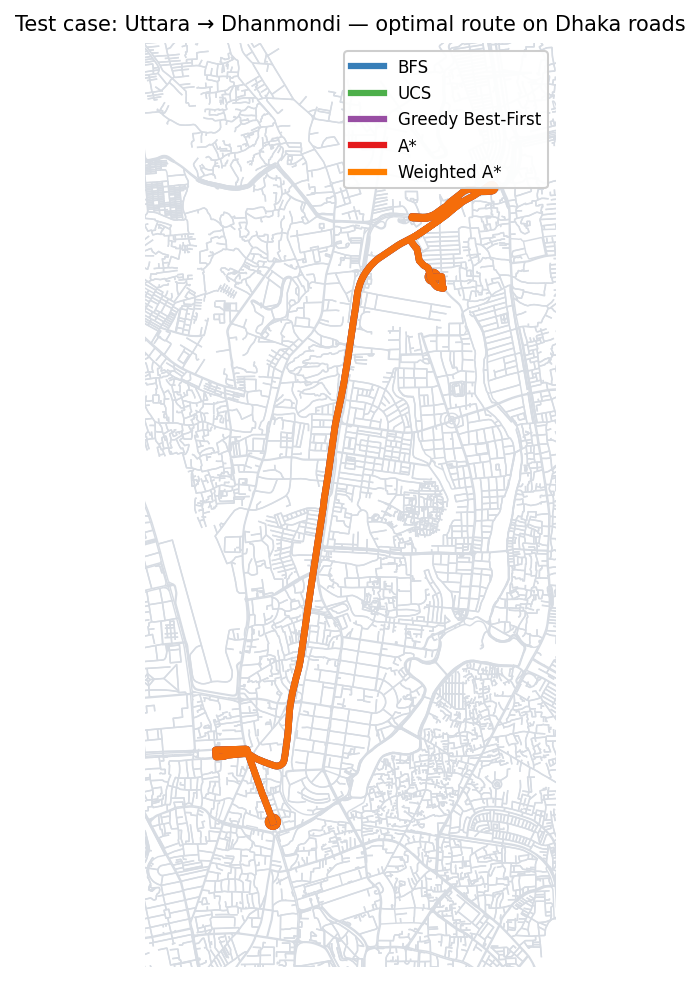
\includegraphics[width=\linewidth]{figures/a1_routes_algorithms.png}
    \caption{All algorithms on the same scenario: cost-optimal methods (A$^\ast$, UCS, W-A$^\ast$, greedy) overlap on one corridor; colours are stacked so only the top-drawn is visible.}
    \label{fig:a1route}
  \end{subfigure}\hfill
  \begin{subfigure}{0.48\linewidth}
    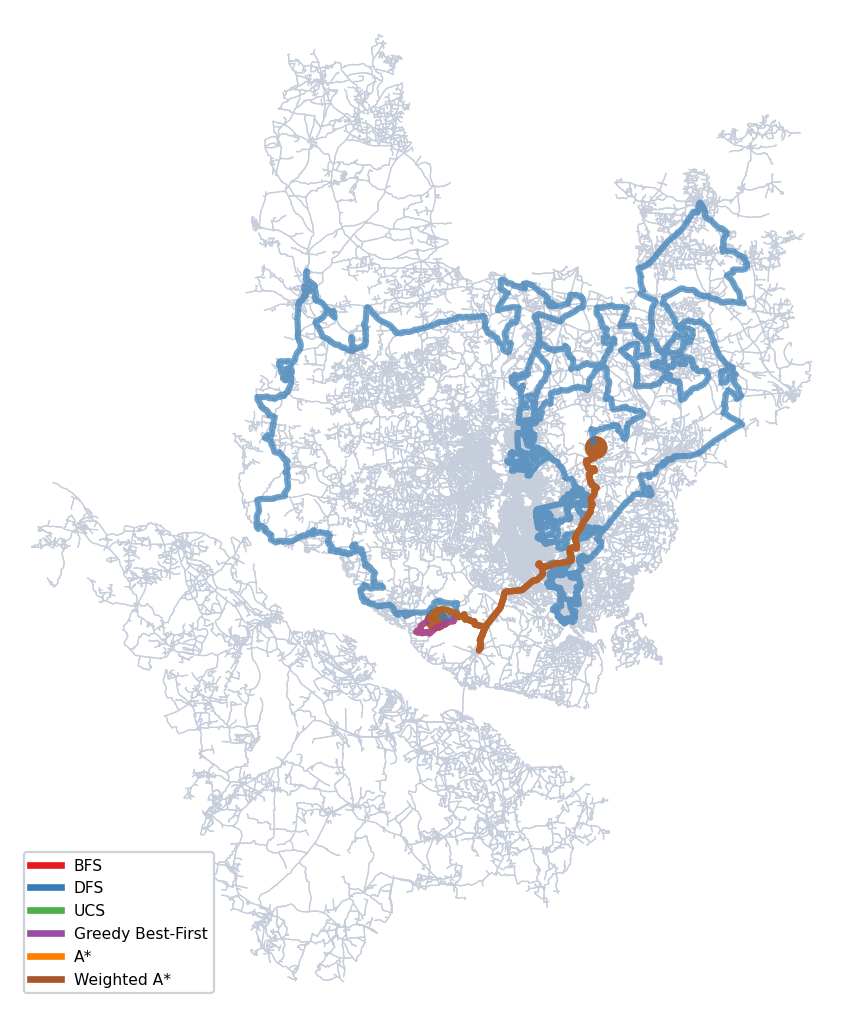
\includegraphics[width=\linewidth]{figures/a1_all_routes.png}
    \caption{DFS (blue) wanders across almost the entire city while all informed methods share a short, direct corridor same scenario, starkly different paths.}
    \label{fig:a1allroutes}
  \end{subfigure}
  \caption{Worked test case (Uttara $\rightarrow$ Dhanmondi, car, evening peak). \emph{Left}: route overlap of cost-aware methods. \emph{Right}: DFS vs.\ informed methods the cost of ignoring both $g$ and $h$ made visible.}
  \label{fig:a1testcase}
\end{figure}

\begin{table}[H]
\centering
\small
\begin{tabularx}{\linewidth}{@{}lXrrr@{}}
\toprule
Algorithm & Found & Cost & Expanded & Runtime (ms) \\
\midrule
Greedy best-first & yes & $16{,}103$ & $\mathbf{41}$   & $1.4$ \\
Weighted $\text{A}^\ast$ & yes & $16{,}103$ & $41$   & $1.3$ \\
$\text{A}^\ast$   & yes & $\mathbf{16{,}103}$ & $196$  & $8.0$ \\
UCS               & yes & $\mathbf{16{,}103}$ & $6{,}524$ & $284$ \\
BFS               & yes & $16{,}103$ & $7{,}218$ & $130$ \\
IDDFS             & yes & $\mathbf{16{,}103}$ & $537{,}716$ & $12{,}131$ \\
DFS               & yes & $3{,}241{,}926$ & $23{,}322$ & $563$ \\
\bottomrule
\end{tabularx}
\caption{Per-algorithm outcome on the worked test case (single query, Setup~1, balanced profile). The five cost-aware methods return the same optimal route ($16{,}103$) with vastly different effort; IDDFS also reaches the optimum here (the goal lies within its $40$-edge depth cap) but only after expanding ${\sim}5.4\times10^{5}$ nodes over $12$\,s, and DFS commits to the first deep branch and returns a route ${\sim}201\times$ costlier.}
\label{tab:a1testcase}
\end{table}


\paragraph{Aggregate Analysis:} 
\mbox{}\\
We now analyse the $10$-scenario averages along four dimensions: solution quality, search effort, heuristic informativeness, and runtime together with robustness. \Cref{tab:a1setup1} reports Setup~1.

\paragraph{Solution quality (optimality).}
The cost column follows theory exactly. UCS and $\text{A}^\ast$ are the only optimal methods and return an identical cost of $44{,}935$. Weighted $\text{A}^\ast$ ($45{,}474$, $+1.2\%$) and greedy ($46{,}328$, $+3.1\%$) are mildly sub-optimal, the price of inflating or relying solely on $h$. BFS ($45{,}943$) minimizes the number of hops rather than cost and only accidentally lands near the optimum. DFS is catastrophic at $2.86\times10^{6}$ roughly $64\times$ the optimum because it commits to the first path it finds regardless of cost. This cleanly reproduces the completeness/optimality hierarchy of the search literature~\citep{russell2021ai}.

\paragraph{Search effort.}
The headline efficiency result is that $\text{A}^\ast$ attains the \emph{same} optimum as UCS while expanding only $7{,}519$ nodes versus $35{,}496$ a $4.7\times$ reduction in work purchased entirely by the heuristic. Greedy and Weighted $\text{A}^\ast$ expand the fewest nodes ($\approx2{,}700$) but forfeit optimality; BFS and DFS expand $\approx36{,}000$, exploring almost the whole reachable graph. Thus expansion count and solution quality trade off along a clear frontier, with $\text{A}^\ast$ occupying the optimal-yet-efficient corner.

\begin{table}[H]
\centering
\small
\begin{tabularx}{\linewidth}{@{}Xrrrc@{}}
\toprule
Algorithm & Avg.\ cost & Expanded & Runtime (ms) & Optimal? \\
\midrule
Greedy best-first                         & $46{,}328$          & $2{,}679$  & $84$    & No \\
Weighted $\text{A}^\ast$ ($\omega{=}1.7$) & $45{,}474$          & $2{,}696$  & $88$    & Bounded \\
$\text{A}^\ast$                            & $\mathbf{44{,}935}$ & $7{,}519$  & $355$   & \textbf{Yes} \\
UCS                                       & $\mathbf{44{,}935}$ & $35{,}496$ & $1{,}605$ & \textbf{Yes} \\
BFS                                       & $45{,}943$          & $36{,}392$ & $708$   & No (min-hops) \\
DFS                                       & $2{,}858{,}809$     & $35{,}939$ & $751$   & No \\
IDDFS                                     & --                  & --         & --      & No (depth cap) \\
\bottomrule
\end{tabularx}
\caption{Assignment~1, Setup~1 (admissible reverse-Dijkstra heuristic). Averages over 10 random scenarios. 
IDDFS fails on all scenarios because the goal depth exceeds the edge limit.}
\label{tab:a1setup1}
\end{table}


\paragraph{Heuristic informativeness.}
The role of heuristic quality is isolated by comparing the two setups (\Cref{tab:a1setup2}). 
Under the informative reverse-Dijkstra heuristic, $\text{A}^\ast$ expands $7{,}519$ nodes; under 
the weak Euclidean heuristic blind to traffic and safety, the dominant terms of the cost surface $\text{A}^\ast$ expands $35{,}116$ nodes, essentially collapsing onto UCS. The effect on greedy search is even more dramatic: guided by straight-line distance in a jam- and safety-dominated cost space, greedy is pulled along geometrically short but expensive routes and its average cost explodes from $46{,}328$ to $200{,}686$ ($4.3\times$ worse). This is the assignment's central empirical claim: \emph{a heuristic misaligned with the true cost forfeits the entire advantage of being informed.} \Cref{fig:a1plots}  visualizes the expansion collapse.

\begin{table}[H]
\centering
\small
\begin{tabularx}{\linewidth}{@{}Xrrrr@{}}
\toprule
& \multicolumn{2}{c}{\textbf{Setup~1} (informative $h$)} & \multicolumn{2}{c}{\textbf{Setup~2} (Euclidean $h$)} \\
\cmidrule(lr){2-3}\cmidrule(lr){4-5}
Algorithm & Avg.\ cost & Expanded & Avg.\ cost & Expanded \\
\midrule
Greedy                            & $46{,}328$          & $2{,}679$  & $200{,}686$         & $14{,}830$ \\
Weighted $\text{A}^\ast$ ($\omega{=}1.7$) & $45{,}474$          & $2{,}696$  & $46{,}201$          & $35{,}218$ \\
$\text{A}^\ast$                   & $\mathbf{44{,}935}$ & $7{,}519$  & $\mathbf{44{,}935}$ & $35{,}116$ \\
UCS                               & $\mathbf{44{,}935}$ & $35{,}496$ & $\mathbf{44{,}935}$ & $35{,}496$ \\
BFS                               & $45{,}943$          & $36{,}392$ & $45{,}943$          & $36{,}392$ \\
DFS                               & $2{,}858{,}809$     & $35{,}939$ & $2{,}858{,}809$     & $35{,}939$ \\
IDDFS                             & --                  & --         & --                  & -- \\
\bottomrule
\end{tabularx}
\caption{Setup~1 vs.\ Setup~2: effect of heuristic informativeness on all seven algorithms. 
Informed methods ($\text{A}^\ast$, greedy, W-$\text{A}^\ast$) are most affected; uninformed methods are unchanged.}
\label{tab:a1setup2}
\end{table}


\begin{figure}[H]
  \centering
  \begin{subfigure}{0.48\linewidth}
    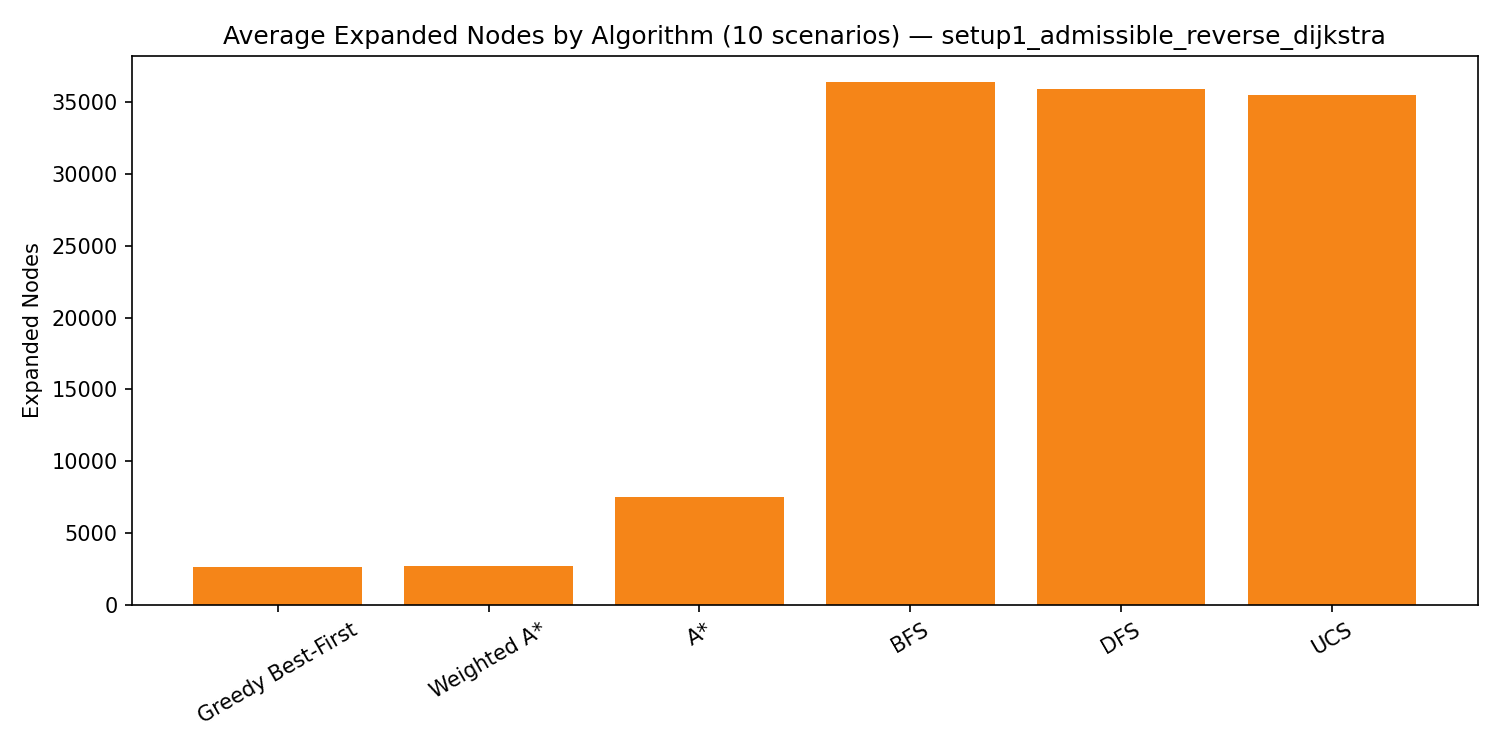
\includegraphics[width=\linewidth]{figures/a1_expanded_setup1.png}
    \caption{Nodes expanded (Setup~1).}
  \end{subfigure}\hfill
  \begin{subfigure}{0.48\linewidth}
    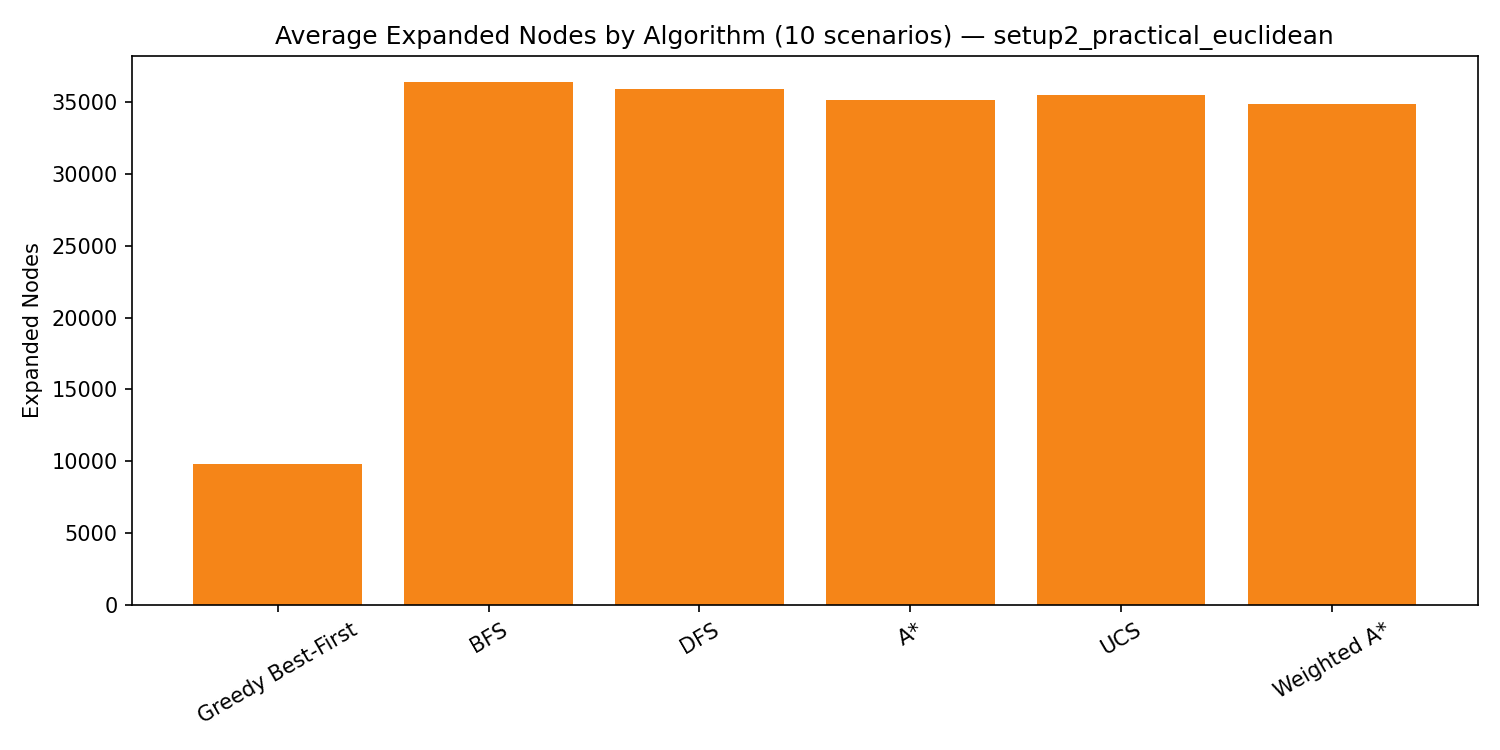
\includegraphics[width=\linewidth]{figures/a1_expanded_setup2.png}
    \caption{Nodes expanded (Setup~2).}
  \end{subfigure}
  \caption{Average nodes expanded per algorithm. A Euclidean heuristic (right) erases the advantage of $\text{A}^\ast$ over UCS visible under the informative heuristic (left).}
  \label{fig:a1plots}
\end{figure}


\paragraph{Runtime.}
Wall-clock time tracks expansion but amplifies it through per-node heuristic look-ups. In Setup~1, $\text{A}^\ast$ ($355$\,ms) is $4.5\times$ faster than UCS ($1{,}605$\,ms); greedy and Weighted $\text{A}^\ast$ are fastest ($\approx85$\,ms). Note that a heuristic is not free: in Setup~2 the added heuristic evaluations make $\text{A}^\ast$ (and even Weighted $\text{A}^\ast$) \emph{slower} than in Setup~1 while expanding as many nodes as UCS an informative heuristic pays for itself, a weak one is pure overhead. \Cref{fig:a1runtime} shows the runtime ranking alongside the solution-cost ranking, in which DFS's cost dwarfs every other method.

\begin{figure}[H]
  \centering
  \begin{subfigure}{0.48\linewidth}
    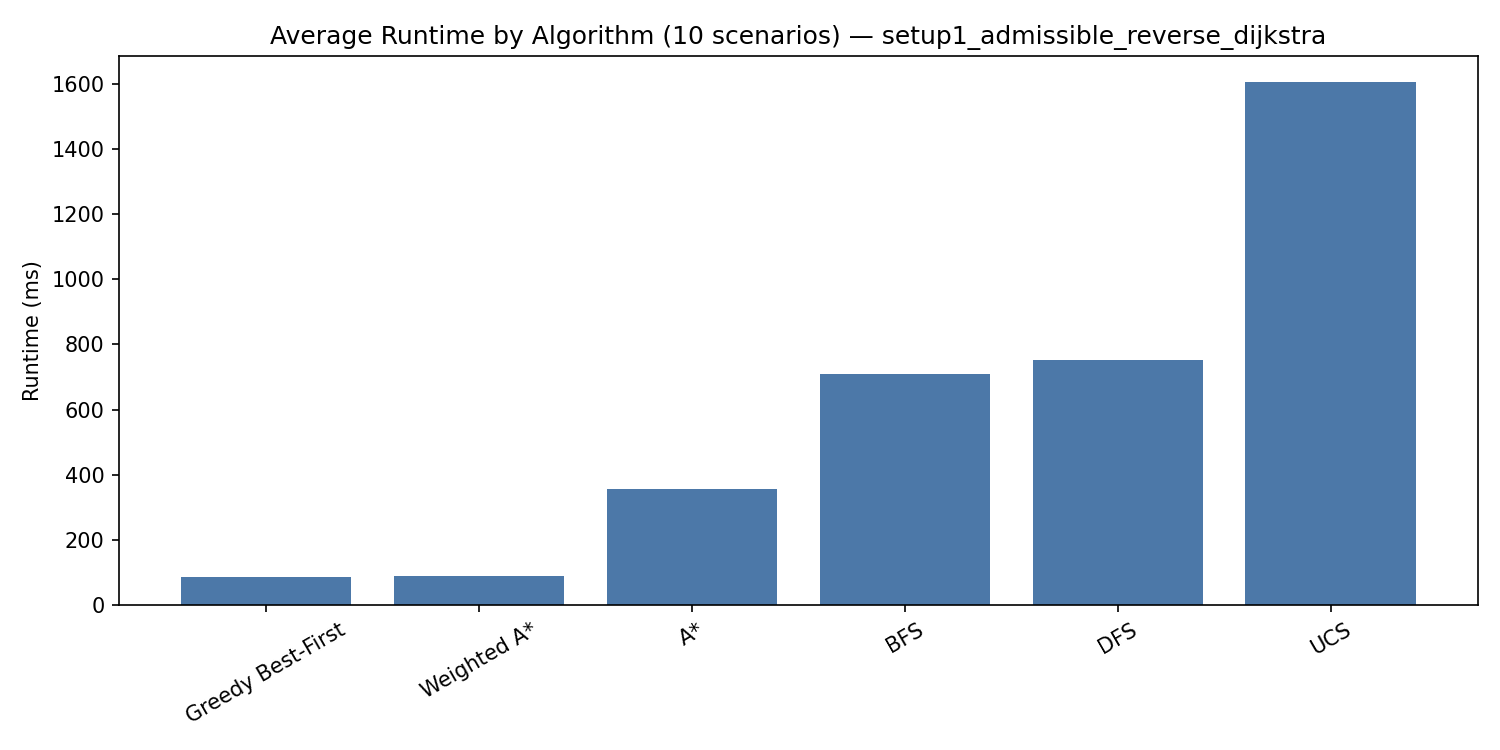
\includegraphics[width=\linewidth]{figures/a1_runtime_setup1.png}
    \caption{Average runtime per algorithm (Setup 1).}
  \end{subfigure}\hfill
  \begin{subfigure}{0.48\linewidth}
    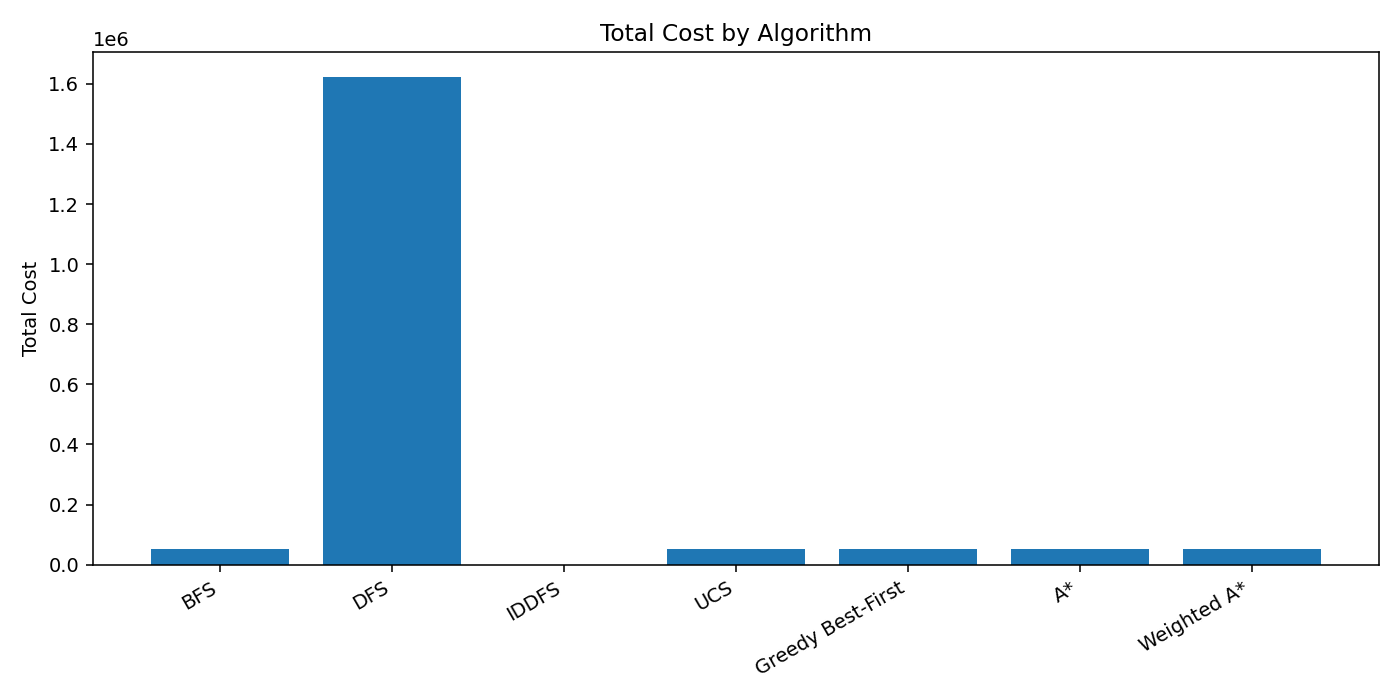
\includegraphics[width=\linewidth]{figures/a1_total_cost.png}
    \caption{Path cost per algorithm (single query).}
  \end{subfigure}
  \caption{Runtime (left) and solution cost (right) by algorithm. $\text{A}^\ast$ reaches the optimum at a fraction of UCS's runtime, while DFS's path cost is orders of magnitude larger than any other method a visual confirmation of its non-optimality.}
  \label{fig:a1runtime}
\end{figure}

\paragraph{Robustness, feasibility, and synthesis.}
The $70\%$ success rate is not solver failure but genuine scenario infeasibility (e.g.\ a bus whose origin is surrounded by narrow roads it cannot legally enter); all cost-based solvers agree on feasibility because they share the same $+\infty$-pruned successor function. A different, \emph{structural} failure affects IDDFS: in every sampled scenario the shortest-hop depth to the goal exceeds its $40$-edge cap, so it returns no path at all a reminder that a fixed depth limit does not transfer to city-scale graphs. Because all figures are averaged over randomized scenarios, the rankings are stable rather than artefacts of a single query, and across all four dimensions the same lesson recurs: $\text{A}^\ast$ with an admissible, \emph{informative} heuristic is the only method that is simultaneously optimal and efficient, and its advantage is exactly proportional to how well the heuristic mirrors the true multi-criteria cost.





\subsection{Key Takeaways and Empirical Synthesis}
\label{sec:a1takeaways}

Our empirical evaluation of the multi-criteria Dhaka routing problem yields three definitive conclusions:

\begin{enumerate}
  \item \textbf{Optimal vs.\ Uninformed Search}: A cost-aware multi-criteria surface renders hop-based metrics obsolete. BFS and DFS ignore edge weights, leading DFS to catastrophic sub-optimality ($64\times$ optimal cost). Only UCS and $\text{A}^\ast$ guarantee exact cost optimality, but $\text{A}^\ast$ achieves it with a $4.7\times$ reduction in node expansions ($7{,}519$ vs.\ $35{,}496$).
  \item \textbf{Importance of Heuristic Alignment}: A heuristic's value lies entirely in its fidelity to the underlying cost surface. Replacing our reverse-Dijkstra lower-bound $h$ with a naive Euclidean baseline (Setup~2) causes $\text{A}^\ast$ to collapse to blind UCS ($35{,}116$ expansions) and degrades Greedy search cost by $4.3\times$ ($200{,}686$). Informed search is only as good as its heuristic's alignment with reality.
  \item \textbf{Practitioner Recommendation}: Weighted $\text{A}^\ast$ ($\omega=1.7$) emerges as the superior operational algorithm for real-time Dhaka navigation. It expands only ${\approx}2{,}700$ nodes (matching Greedy speed at $88$\,ms) while guaranteeing solution quality within $1.2\%$ of the true optimum ($45{,}474$).
\end{enumerate}

While single-agent search solves spatial pathfinding on the urban graph, urban management during crises (such as fuel shortages) introduces multi-agent resource competition with capacity and policy limits. In \Cref{sec:a2}, we transition from single-agent spatial search to multi-user global constraint optimization.

% =====================================================================

\section{Urban Resource Allocation and Fuel Rationing under Spatial Policy Constraints}
\label{sec:a2}\label{sec:csp}

\subsection{Motivation and Problem Formulation}
\label{sec:a2formulation}

Urban fuel crises turn a routine service interaction into a constrained allocation problem where each vehicle has a limited range, 
rationing policies bar it from many stations, and the city's finite station capacities must be shared equitably among all users simultaneously. 
Solving this is a timely and realistic problem on urban area because the legality of any one assignment depends on every other assignment 
station loads and household choices interact globally. 
We formalize the problem as a Constraint Satisfaction and Optimization Problem (CSOP)~\citep{dechter2003constraint,russell2021ai}:

\textbf{Variables.} One variable per user, $X=\{x_1,\dots,x_n\}$; assigning a value to $x_i$ decides where user $i$ fuels. Each user carries fixed attributes a location on the Dhaka road graph, a vehicle class, a license-plate parity, a remaining fuel range, and a fuel demand that shape which values are legal for it.

\textbf{Domains.} Every variable draws its value from the set of fueling stations $S=\{s_1,\dots,s_m\}$, each with a finite capacity; a complete assignment is a map $\sigma:X\to S$, where $\sigma(x_i)=s_j$ means user $i$ fuels at station $j$. The \emph{effective} domain $D_i\subseteq S$ of each variable is what survives the unary constraints below.

\textbf{Constraints.} A set $C$ of nine hard constraints derived from the government rationing policy $\Pi$, grouped by arity: \emph{unary} constraints filter which stations are physically and legally reachable per user; a \emph{binary} anti-hoarding constraint prevents household members from sharing a station; and \emph{global} constraints enforce capacity limits, public-transport reserves, emergency reserves, and fair-service quotas. A full listing with their policy basis appears in \Cref{tab:a2constraints}. An assignment is \emph{feasible} iff every constraint in $C$ is satisfied.

\textbf{Objective.} Among feasible assignments making this a constraint satisfaction \emph{and} optimization problem minimize the dual-criteria soft cost
\begin{equation}
\mathrm{cost}(\sigma)\;=\;w_{d}\!\sum_{x\in X}\mathrm{dist}\big(x,\sigma(x)\big)\;+\;w_{L}\,\operatorname{Var}\!\Big(\big\{\ell_s(\sigma)\big\}_{s\in S}\Big),
\qquad
\ell_s(\sigma)=\frac{\sum_{x\in\sigma^{-1}(s)}\!\mathrm{demand}(x)}{\mathrm{capacity}(s)},
\label{eq:cspcost}
\end{equation}
where the first term penalizes aggregate travel distance and the second penalizes unequal station loading a proxy for preventing 
localized queue overflows onto surrounding roads. The weights $(w_d, w_L)$ and the distance oracle $\mathrm{dist}(\cdot)$ are scenario-dependent 
(Section~\ref{sec:a2env}); \Cref{tab:a2notation} collects all symbols.

\begin{table}[H]
\centering
\small
\begin{tabularx}{\linewidth}{@{}lX@{}}
\toprule
Symbol & Meaning \\
\midrule
$X,\,n$           & set of users / number of users \\
$S,\,m$           & set of fueling stations / number of stations \\
$D_i \subseteq S$ & legal-station domain for user $x_i$ after unary filtering \\
$\sigma(x)$       & station assigned to user $x$ \\
$\ell_s(\sigma)$  & demand-to-capacity load ratio at station $s$ \\
$(w_d,\,w_L)$     & cost weights for travel distance and load variance \\
$\Pi$             & government rationing policy (parity, reserves, caps, quotas) \\
\bottomrule
\end{tabularx}
\caption{Assignment~2 notation.}
\label{tab:a2notation}
\end{table}

We treat this study as a controlled empirical evaluation of CSP-solving strategies, analysed in \Cref{sec:a2results}. 

\textbf{First}, whether variable-ordering (MRV, degree), value-ordering (LCV), forward checking, and AC-3 arc consistency convert intractable naive 
backtracking into a practical solver. 
\textbf{Second}, at what problem scale $n$ systematic backtracking becomes infeasible, and whether local search (Min-Conflicts) extends 
tractability beyond that point. 
\textbf{Third}, how severely aggressive rationing shrinks the feasible domain, and what fraction of users it renders unserviceable on a city-scale instance.



\subsection{Methodology}

\subsubsection{Simulation Environment and Rationing Model}
\label{sec:a2env}
The world is built from two real data sources. The Dhaka road network is loaded from \emph{OpenStreetMap} via the \textsf{OSMnx} library~\citep{boeing2017osmnx}, represented as a directed graph whose \emph{nodes} are intersections and whose \emph{edges} are road segments carrying their true length and OSM \texttt{highway} class. Real fueling stations are queried directly from OSM using the tag \texttt{amenity=fuel}; because OSM does not record pump capacities, these are synthesized from a parametric distribution (values and rationale in \Cref{sec:a2defend}).

Each \emph{user} $x_i \in X$ is a synthetic vehicle generated at a random road-network node, characterized by four attributes: a vehicle class (private car, public bus/CNG, or emergency vehicle), a license plate parity (odd or even), a remaining fuel range (determining how far the user can travel to reach a station), and a volumetric fuel demand. Vehicle class splits and demand ranges are design choices motivated by Dhaka's fleet composition; they are stated and justified in \Cref{sec:a2defend}.

A per-(vehicle-class, station) \emph{distance oracle} is pre-computed by reverse Dijkstra on a vehicle-aware edge weight: road-type restrictions (wide vs.\ narrow) and a time-of-day traffic scaling are baked into the edge weight so that the oracle reflects true reachability, not straight-line distance. Reachability constraint U1 holds for user $x_i$ at station $s$ iff this oracle distance does not exceed $x_i$'s remaining fuel range. \Cref{tab:a2constraints} lists all nine constraints that filter and shape the feasible space.

\begin{table}[H]
\centering
\small
\begin{tabularx}{\linewidth}{@{}llXl@{}}
\toprule
ID & Type & Enforces & Policy basis \\
\midrule
U1 & unary  & user can reach station within remaining fuel range & physical reachability \\
U2 & unary  & a fraction of stations serve emergency vehicles only & emergency access \\
G1 & unary  & odd/even plate day bars off-parity civilian vehicles & 2022 rationing~\citep{thewire2022fuel} \\
G6 & unary  & CNG stations close to civilian traffic during peak hours & Dhaka CNG policy \\
B1 & binary & household members must refuel at \emph{different} stations & anti-hoarding \\
G3 & global & reserve a fraction of civilian capacity for public transport & keep buses running \\
G4 & global & lock a fraction of capacity for emergency vehicles & strategic reserve \\
G8 & global & at most $q_{\max}$ users queued per station & avoid road-blocking queues \\
G9 & global & each station must serve at least one user & equitable coverage \\
\bottomrule
\end{tabularx}
\caption{The nine constraints, grouped by arity, with the real-world rationing lever each encodes. Values and justification appear in \Cref{sec:a2defend}.}
\label{tab:a2constraints}
\end{table}

\subsubsection{Design Rationale and Empirical Basis}
\label{sec:a2defend}

A constraint model is only as credible as the reasoning behind its rules, so we justify each design choice rather than merely assert it.

\paragraph{(i) Plate-parity rationing (G1).} Odd/even plate-day restrictions are a well-documented tool for managing acute fuel shortages. During the 2022 Bangladesh fuel crisis, surging global oil prices forced the government to close filling stations one day per week and later impose plate-parity scheduling to reduce queue lengths, which had grown long enough to block surrounding traffic~\citep{thewire2022fuel,dailystar2022fuelration}. We encode this as a hard unary filter: on a designated parity day, all off-parity civilian vehicles have their domain pruned to the empty set, forcing the solver to declare them unserviceable an honest representation of the policy's effect.

\paragraph{(ii) Emergency-station exclusivity (U2).} We designate a fraction of stations as exclusive to emergency fleets (ambulances, fire engines, police). The motivation is the documented concern that during the 2022 crisis, petrol stations serving mixed traffic created dangerous delays for emergency vehicles~\citep{dailystar2022fuelration}. Setting $8\%$ of stations as emergency-only is a conservative estimate; the parameter is fully tunable. This is modelled as a unary filter that removes non-emergency users from those stations' domains before search begins.

\paragraph{(iii) Peak-hour CNG closures (G6).} Dhaka's CNG refueling network operates under periodic civilian restrictions during peak commute hours, a policy used to prioritise fuel for the auto-rickshaw and taxi fleet that serves bulk passenger transport~\citep{tbs2023cctv}. We implement this as a unary constraint that closes CNG-type stations to private vehicles during designated time slots. Because CNG stations constitute approximately $35\%$ of queried OSM stations, this constraint materially shrinks domain sizes.

\paragraph{(iv) Anti-hoarding binary constraint (B1).} During fuel crises, household stockpiling is a primary driver of queue overflows. To model the anti-hoarding regulation, vehicles sharing a household cannot be assigned to the same station ($x_i \neq x_j$ for household peers). This is the only binary constraint in the problem and is the reason AC-3 arc consistency is applied: household relationships form a sparse constraint graph that propagates domain pruning across household pairs before search begins.

\paragraph{(v) Capacity reserves: public transport (G3) and emergency (G4).} Two global constraints carve out fixed fractions of each station's civilian capacity. Reserving $60\%$ for public-transport vehicles (G3) reflects the government priority of keeping buses and shared taxis running during a supply shock, since these carry far more passengers per litre than private cars. The $10\%$ strategic emergency reserve (G4) is a standard civil-defence buffer. Both fractions are design choices calibrated to make the constraints clearly binding (not trivially satisfied) on our synthetic fleet; they can be replaced by any empirically derived reserve requirement without changing the solver logic.

\paragraph{(vi) Queue cap (G8) and fair-service quota (G9).} Queue lengths at fuel stations during the 2022 crisis were reported to block surrounding roads, disrupting traffic for hours~\citep{dailystar2022fuelration}. We enforce a maximum queue of $q_{\max}=8$ concurrent users per station as a global capacity constraint, chosen to be plausibly tight but not trivially infeasible on our instance sizes. The fair-service quota (G9) requires every station to serve at least one user, preventing degenerate solutions that overload a single central station.

\paragraph{On the simulation framing.} Station capacities are synthesized from a $2000\,\mathrm{L}\pm40\%$ distribution, reflecting 
realistic variation between small neighbourhood pumps and large arterial stations; the $\pm40\%$ jitter injects per-scenario variability 
analogous to the random noise in Assignment~1's cost surface. User vehicle-class proportions ($60\%$ private, $30\%$ public, $10\%$ emergency), 
fuel ranges, and demand levels are calibrated to produce a fleet that stresses all nine constraints simultaneously not to replicate a specific census. 
The cost weights $(w_d, w_L)=(1, 500)$ are set so that load variance dominates distance: a solution that evenly distributes demand across all 
stations is always preferred over one that concentrates load even if individual trips are slightly shorter. 

 Value above station capacities, vehicle-class proportions, fuel ranges, demand levels, the queue cap, and the cost weights is a transparent, tunable design choice, not a measured Dhaka quantity, and each can be replaced by a calibrated real-data estimate without touching the solvers or the evaluation code. As in the earlier assignments, our conclusions therefore depend only on the relative orderings between solver configurations, not on the absolute cost magnitudes.


\subsubsection{From Rationing Policy to Fuel Allocation: The Algorithmic Approach}

The three solvers share the same preprocessed problem; they differ only in how they search it. We make that split precise before describing each one.

Before any solver runs, two preprocessing passes reduce the domains. First, \emph{unary filtering} removes stations that violate constraints U1, U2, G1, and G6 for each user independently. Second, \emph{AC-3 arc consistency}~\citep{mackworth1977consistency} is applied to the one binary constraint B1 (household anti-hoarding): for every pair of household members $(x_i, x_j)$, any station value $v \in D_i$ that has no compatible counterpart in $D_j$ is pruned. This propagates through household chains and can trigger domain wipe-outs that prove inconsistency before search even starts (\Cref{alg:ac3}). All three solvers then receive the same \emph{post-filtering} domains $D'$; the difference lies entirely in \emph{how} they search within them.

\begin{algorithm}[H]
\caption{AC-3 arc consistency for the household not-equal constraint (B1).}
\label{alg:ac3}
\begin{algorithmic}[1]
\State $Q\gets$ all arcs $(x_i,x_j)$ such that $x_i,x_j$ share a household
\While{$Q\neq\emptyset$}
  \State $(x_i,x_j)\gets\textsc{Dequeue}(Q)$
  \If{\Call{Revise}{$x_i,x_j$}}
    \If{$D_i=\emptyset$} \Return \textsc{Inconsistent}
    \EndIf
    \ForAll{$x_k$ in $x_i$'s household, $x_k\neq x_j$} \State $\textsc{Enqueue}(Q,(x_k,x_i))$
    \EndFor
  \EndIf
\EndWhile
\State \Return \textsc{Consistent}
\Statex
\Function{Revise}{$x_i,x_j$}
  \State drop from $D_i$ every $v$ with no $w\in D_j$ s.t.\ $w\neq v$;\ \ \Return whether $D_i$ shrank
\EndFunction
\end{algorithmic}
\end{algorithm}


\paragraph{What the cost function adds and where it enters.}
The soft objective $\mathrm{cost}(\sigma)$ from \cref{eq:cspcost} is \emph{invisible} to systematic backtracking: backtracking returns the \emph{first} complete consistent assignment it finds, not the minimum-cost one. Min-Conflicts, by contrast, directly minimizes a conflict count that acts as a proxy for constraint violations and since the repair move selects the station that \emph{minimizes violations}, it implicitly tends toward load-balanced assignments that also reduce $\mathrm{cost}(\sigma)$. This asymmetry is one reason Min-Conflicts yields slightly lower cost than backtracking on feasible instances (\Cref{sec:a2results}).

\paragraph{The solver configurations.}
The table below shows what each configuration uses, mirroring the search-key table of Assignment~1:

{\small
\begin{tabularx}{\linewidth}{@{}llcll@{}}
\toprule
Solver & Strategy & AC-3 & Heuristics & Cost-optimal? \\
\midrule
Naive BT       & DFS, no ordering        & \checkmark &                    & No (first feasible) \\
Heuristic BT   & DFS + MRV/deg/LCV + FC  & \checkmark & MRV, degree, LCV     & No (first feasible) \\
Min-Conflicts  & local repair + restart  & $\checkmark^{*}$ &             & No (violation proxy) \\
\bottomrule
\multicolumn{5}{@{}l}{\footnotesize $^{*}$AC-3 as pre-filter only.}
\end{tabularx}}

\paragraph{Variable and value-ordering.}
In CSP backtracking, the analogous role is played by variable- and value-ordering heuristics: \textbf{MRV} (Minimum Remaining Values) selects the variable most constrained by current assignments the one most likely to fail first so dead ends are detected early rather than after many nodes have been expanded. The \textbf{degree} heuristic breaks MRV ties by choosing the variable involved in the most constraints on remaining unassigned peers, propagating pruning effects most widely. \textbf{LCV} (Least Constraining Value) then orders station choices so that the assigned value rules out the fewest options for other variables the mirror of $h$ in that it looks \emph{forward} to preserve flexibility. Together, these heuristics compress the effective branching factor without changing the correctness guarantee of backtracking.

Now lets focus on the three solver configurations in detail.

\paragraph{Solver 1: Backtracking (naive and heuristic).}
Systematic depth-first assignment (\Cref{alg:backtrack}). In its \emph{naive} form it assigns values with no ordering: complete if a solution exists it is found but its effort grows as $O(d^n)$ in the worst case, so it is tractable only on small instances and serves as our baseline. The \emph{heuristic} form augments the same DFS with the MRV, degree, and LCV orderings described just above, plus \emph{forward checking}, which prunes the chosen station from household neighbours' domains and fails early if any domain empties. These heuristics leave completeness and optimality untouched; they only compress the effective branching factor, and how much they compress it on our nine-constraint problem is the first thing the experiments measure.

\begin{algorithm}[H]
\caption{Backtracking search with MRV\,+\,degree\,+\,LCV\,+\,forward checking.}
\label{alg:backtrack}
\begin{algorithmic}[1]
\Function{Backtrack}{$\sigma$}
  \If{$\sigma$ is complete} \Return $\sigma$
  \EndIf
  \State $x\gets\textsc{SelectVar}$ \Comment{MRV, tie-broken by degree}
  \ForAll{$s\in\textsc{OrderValues}(x)$} \Comment{LCV order}
    \If{$s$ is consistent with $\sigma$ (B1, G3, G4, G8)}
      \State add $x\!\mapsto\!s$;\ \ \textsc{ForwardCheck} (prune neighbours)
      \If{no domain became empty}
        \State $r\gets$\Call{Backtrack}{$\sigma$};\ \ \textbf{if} $r\neq$ failure \textbf{return} $r$
      \EndIf
      \State undo $x\!\mapsto\!s$ and its pruning \Comment{backtrack}
    \EndIf
  \EndFor
  \State \Return failure
\EndFunction
\end{algorithmic}
\end{algorithm}

\paragraph{Solver 2: Min-Conflicts local search.}
Min-Conflicts (\Cref{alg:minconflicts}) abandons systematic search for local repair~\citep{minton1992minconflicts}: from a random complete assignment it repeatedly moves a randomly chosen conflicted user to the station that minimizes the total violation count, restarting on plateaus. It is neither complete nor optimal, 
but it scales to instances far beyond systematic search. Because its repair move is violation-driven, it implicitly also reduces the load-variance component of $\mathrm{cost}(\sigma)$, so it tends to return slightly lower soft cost than backtracking on feasible instances.

\begin{algorithm}[H]
\caption{Min-Conflicts local search (with random restart).}
\label{alg:minconflicts}
\begin{algorithmic}[1]
\State $\sigma\gets$ random complete assignment (each user a random legal station)
\For{$step=1$ to $\mathit{max\_steps}$}
  \If{$\textsc{Violations}(\sigma)=0$} \Return $\sigma$
  \EndIf
  \State $x\gets$ a randomly chosen user currently in conflict
  \State $\sigma(x)\gets\arg\min_{s\in D_x}\textsc{Violations}\big(\sigma\ \text{with}\ x\!\mapsto\!s\big)$ \Comment{ties random}
  \State on a plateau, perform a random restart
\EndFor
\State \Return best-so-far $\sigma$
\end{algorithmic}
\end{algorithm}

\Cref{tab:a2solvers} contrasts the formal properties of the three solver configurations, in the spirit of the complexity table of Assignment~1.

\begin{table}[H]
\centering
\small
\begin{tabularx}{\linewidth}{@{}lXccX@{}}
\toprule
Solver & Strategy & Complete? & Cost-optimal? & Effort / regime \\
\midrule
Naive backtracking & systematic DFS, no heuristics & Yes & No (first feasible) & $O(d^{n})$ worst case; small $n$ only \\
Heuristic backtracking & DFS + MRV/degree/LCV + FC + AC-3 & Yes & No & far smaller effective branching; medium $n$ \\
Min-Conflicts & local repair from a random start & No & No & $\sim\!O(\text{steps}\cdot n\cdot d)$; large $n$ \\
\bottomrule
\end{tabularx}
\caption{Properties of the three solver configurations ($n$: users, $d$: maximum domain size).}
\label{tab:a2solvers}
\end{table}

\subsubsection{Evaluation Metrics and Experimental Protocol}
This study records metrics that separate correctness, quality, and effort: \textbf{feasibility} 
(solution found vs.\ timeout); \textbf{cost} \cref{eq:cspcost}; \textbf{search effort}, measured as 
\emph{backtracks} for systematic search and \emph{repair iterations} for Min-Conflicts; \textbf{runtime} (ms); and \textbf{users served / unassignable}.

We run three studies plus an ablation: (A)~a head-to-head on a small instance; (B)~a scaling sweep $n\in\{10,20,40,80,160\}$; (C)~a realistic full-Dhaka instance ($150$ users, $30$ stations); and a \emph{three-way} comparison naive backtracking (heuristics off), heuristic backtracking, and Min-Conflicts on identical instances of increasing size. The overall workflow is summarized in \Cref{fig:a2workflow}.

\begin{figure}[H]
  \centering
  \begin{tikzpicture}[
    node distance=1.5cm and 0.55cm,
    every node/.style={draw, rounded corners, align=center,
      minimum width=2.05cm, minimum height=0.7cm, fill=blue!5, font=\small},
    >=Latex]
    \node (g) {OSM Dhaka\\graph};
    \node (u) [right=of g] {Users \& stations\\(policy $\Pi$)};
    \node (f) [right=of u] {Domain filter\\(unary\,+\,AC-3)};
    \node (s) [right=of f] {Solvers\\(BT / Min-Confl.)};
    \node (o) [right=of s] {Assignment\\+ metrics};
    \draw[->,thick] (g) -- (u);
    \draw[->,thick] (u) -- (f);
    \draw[->,thick] (f) -- (s);
    \draw[->,thick] (s) -- (o);
  \end{tikzpicture}
  \caption{Workflow: users and stations under rationing policy $\Pi$ are domain-filtered by unary constraints and AC-3, then solved by systematic backtracking or Min-Conflicts local search.}
  \label{fig:a2workflow}
\end{figure}

\subsection{Results and Discussion}
\label{sec:a2results}

\paragraph{Worked test case}
\mbox{}\\
\textbf{Scenario.} A small Dhanmondi scenario consisting of $12$ users and $8$ stations (Study~A, head-to-head instance). The stations have a baseline capacity of $2000$\,L $\pm 40\%$. Unary filtering and AC-3 are pre-applied to prune initial domains.

\textbf{What we observe.} Due to aggressive rationing policy constraints (such as plate-parity and capacity reserves), only $8$ of the $12$ users are servable, leaving $4$ users unassignable due to domain wipe-outs. Both solvers successfully find a feasible assignment for the servable subset. Backtracking search finds the solution in $0.14$\,ms, expanding $9$ nodes with $0$ backtracks, and returns a load-balanced assignment at a cost of $30{,}295$. Min-Conflicts local search solves the same instance in $0.03$\,ms, requiring only a single repair iteration to converge on a slightly lower cost of $29{,}253$ due to direct optimization of the soft objective \cref{eq:cspcost}. The results are summarized in \Cref{tab:a2testcase}; the resulting station loads are verified in \Cref{fig:a2loads}, and this assignment is mapped onto real Dhaka roads in \Cref{fig:a2} (left).

\begin{table}[H]
\centering
\small
\begin{tabular}{@{}lcrrrc@{}}
\toprule
Solver & Found? & Cost & Served / Unassign. & Effort & Runtime (ms) \\
\midrule
Backtracking (MRV+LCV+FC) & Yes & $30{,}295$ & $8$ / $4$ & $9$ nodes & $0.14$ \\
Min-Conflicts             & Yes & $29{,}253$ & $8$ / $4$ & $1$ iter  & $0.03$ \\
\bottomrule
\end{tabular}
\caption{Solver performance on the Dhanmondi worked test case (12 users, 8 stations; Study~A).}
\label{tab:a2testcase}
\end{table}

\begin{figure}[H]
  \centering
  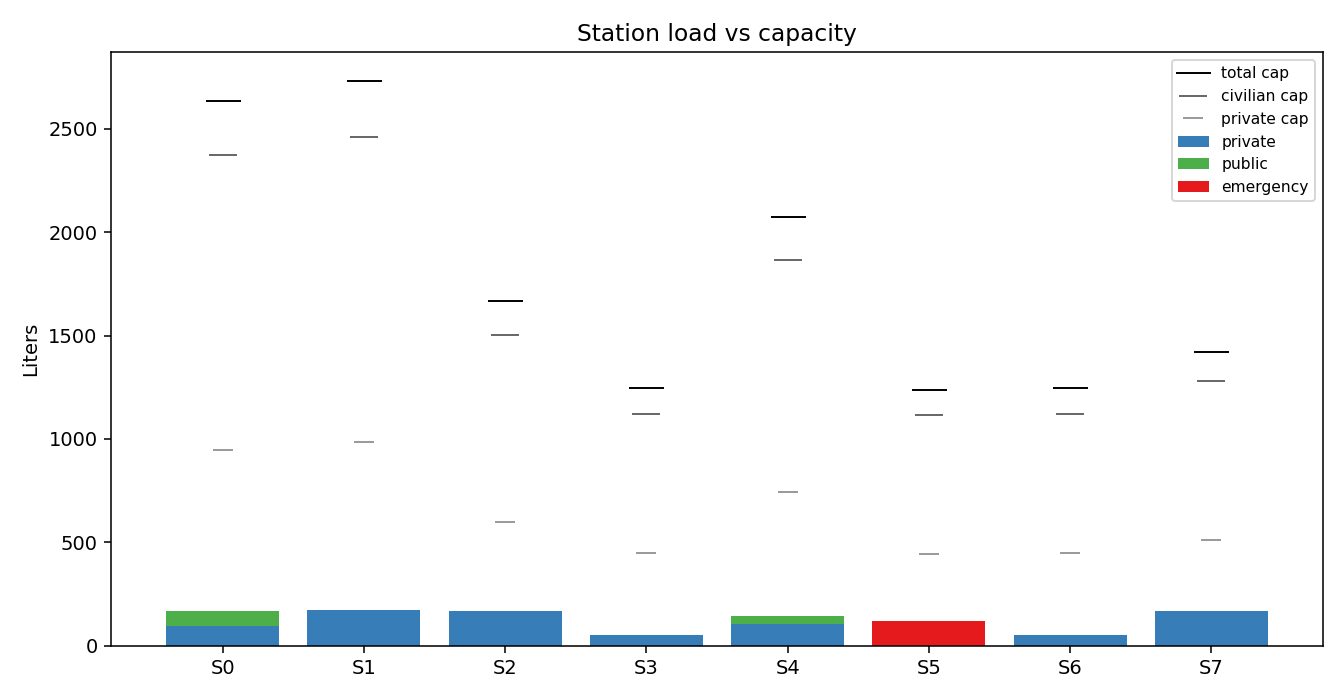
\includegraphics[height=5.2cm]{figures/a2_bt_loads.png}
  \caption{Per-station demand vs.\ capacity under the backtracking assignment (worked example). The private/public/emergency stacks stay within each station's civilian cap and strategic reserve, i.e.\ constraints G3/G4/G8 hold.}
  \label{fig:a2loads}
\end{figure}

\paragraph{A. Heuristic Benefit and Solver Comparison.}
The three-way comparison (\Cref{tab:a2threeway}) evaluates naive backtracking (heuristics off), heuristic backtracking, and Min-Conflicts on identical instances of increasing size. For small instances ($n\le40$), all three methods solve instantly with zero backtracks. At $n=70$, naive backtracking collapses under the combinatorial weight, timing out after $601{,}618$ backtracks. In contrast, heuristic backtracking solves the same instance in $4.12$\,ms with \emph{zero} backtracks, demonstrating the efficiency of MRV and forward checking. At $n=100$, even heuristic backtracking times out as systematic search cannot escape the exponential scaling, while Min-Conflicts returns a high-quality approximate assignment in $957$\,ms. This highlights the classic trade-off: systematic search guarantees completeness but is exponential, while local search scales to larger regimes~\citep{minton1992minconflicts}.

\begin{table}[H]
\centering
\small
\begin{tabularx}{\linewidth}{@{}rXXX@{}}
\toprule
$n$ & Naive backtracking & Heuristic backtracking & Min-Conflicts \\
\midrule
$8$   & solved, $0$ bt, $0.08$\,ms & solved, $0$ bt, $0.12$\,ms & solved, $2$ it, $0.10$\,ms \\
$20$  & solved, $0$ bt & solved, $0$ bt & solved, $1$ it \\
$40$  & solved, $0$ bt & solved, $0$ bt & solved, $1$ it \\
$70$  & \textbf{timeout}, $601{,}618$ bt & solved, $0$ bt, $4.12$\,ms & solved, $4$ it, $0.99$\,ms \\
$100$ & \textbf{timeout} & \textbf{timeout}, $150{,}549$ bt & approx., $3{,}136$ it, $957$\,ms \\
\bottomrule
\end{tabularx}
\caption{Assignment~2 three-way comparison (Study~A). ``bt'' = backtracks, ``it'' = Min-Conflicts iterations.}
\label{tab:a2threeway}
\end{table}

\paragraph{Heuristic Component Analysis.}
To isolate each heuristic's contribution, we run an ablation study by adding them cumulatively on a hard, \emph{over-constrained (infeasible)} instance (\Cref{tab:a2ablation}). MRV and the degree heuristic prune about $6\%$ of backtracks by identifying domain failures early. However, adding LCV and forward checking does not reduce backtracks further on this infeasible instance, instead increasing runtime due to per-node overhead. This contrast is instructive: on a feasible instance, heuristics guide the search directly to a solution (\Cref{tab:a2threeway}), but on an infeasible instance, the search space must be fully exhausted. Ordering heuristics (LCV) and lookahead (FC) accelerate finding solutions, but do not speed up proving their absence.

\begin{table}[H]
\centering
\small
\begin{tabularx}{\linewidth}{@{}Xrr@{}}
\toprule
Configuration & Backtracks & Runtime (ms) \\
\midrule
naiv backtracking & $121{,}545$ & $9{,}001$ \\
$+$ MRV $+$ degree & $114{,}504$ & $9{,}901$ \\
$+$ LCV            & $114{,}504$ & $12{,}365$ \\
$+$ forward checking & $114{,}504$ & $13{,}025$ \\
\bottomrule
\end{tabularx}
\caption{Heuristic ablation on a hard (infeasible) instance, heuristics added cumulatively.}
\label{tab:a2ablation}
\end{table}



\paragraph{B. Systematic vs.\ Local Search at Scale.}
The scaling sweep (\Cref{tab:a2scaling}, \Cref{fig:a2scaling}) measures performance for $n \in \{10, 20, 40, 80, 160\}$ on a larger multi-area bounding box. Where both solvers succeed, Min-Conflicts is consistently faster (e.g., $2.60$\,ms vs.\ $9.99$\,ms at $n=160$) and returns solutions of comparable or slightly lower cost. While both runtimes scale smoothly in this range, the three-way comparison shows that systematic search hits a wall between $n=70$ and $n=100$, whereas local search scales reliably.

\begin{table}[H]
\centering
\small
\begin{tabularx}{\linewidth}{@{}Xrrrr@{}}
\toprule
$n$ & BT time (ms) & MC time (ms) & BT cost & MC cost \\
\midrule
$10$  & $0.07$ & $0.02$ & $20{,}882$  & $20{,}941$ \\
$20$  & $0.18$ & $0.03$ & $52{,}439$  & $52{,}722$ \\
$40$  & $0.66$ & $0.16$ & $119{,}093$ & $125{,}316$ \\
$80$  & $1.85$ & $0.39$ & $296{,}237$ & $282{,}730$ \\
$160$ & $9.99$ & $2.60$ & $691{,}841$ & $638{,}971$ \\
\bottomrule
\end{tabularx}
\caption{Assignment~2 scaling sweep (Study~B): runtime and cost of backtracking (BT) vs.\ Min-Conflicts (MC).}
\label{tab:a2scaling}
\end{table}

\begin{figure}[H]
  \centering
  \begin{subfigure}{0.48\linewidth}
    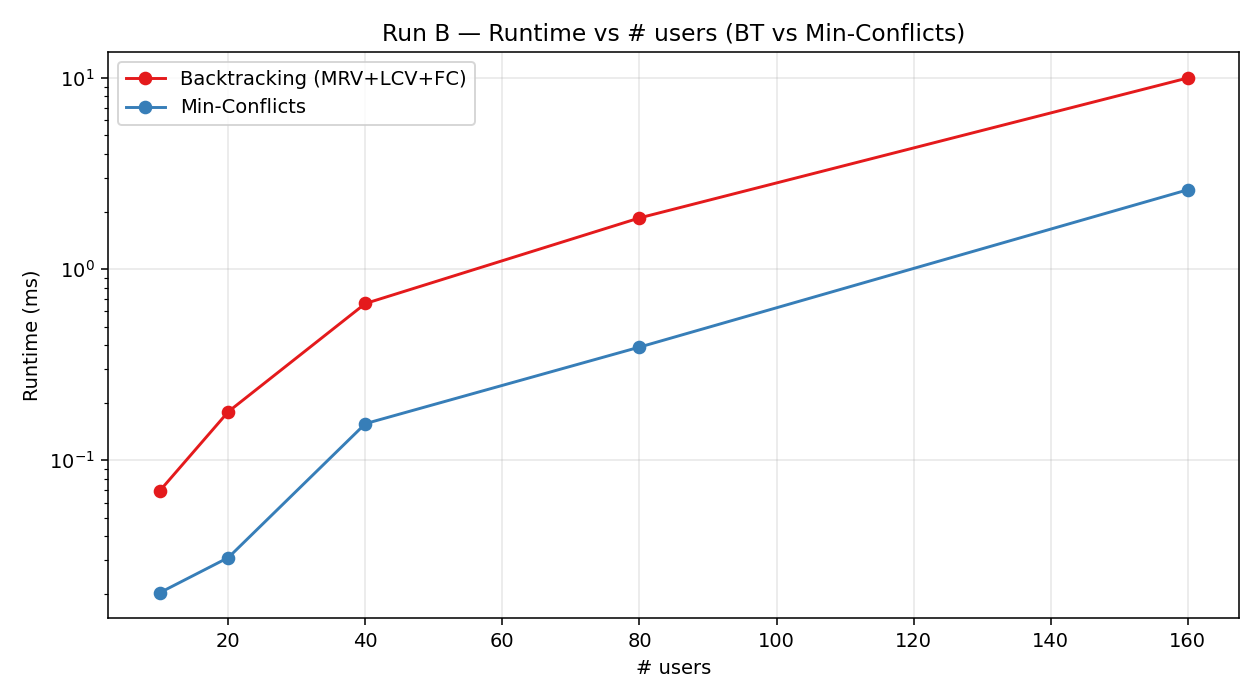
\includegraphics[width=\linewidth]{figures/a2_scaling_runtime.png}
    \caption{Runtime vs.\ number of users $n$.}
  \end{subfigure}\hfill
  \begin{subfigure}{0.48\linewidth}
    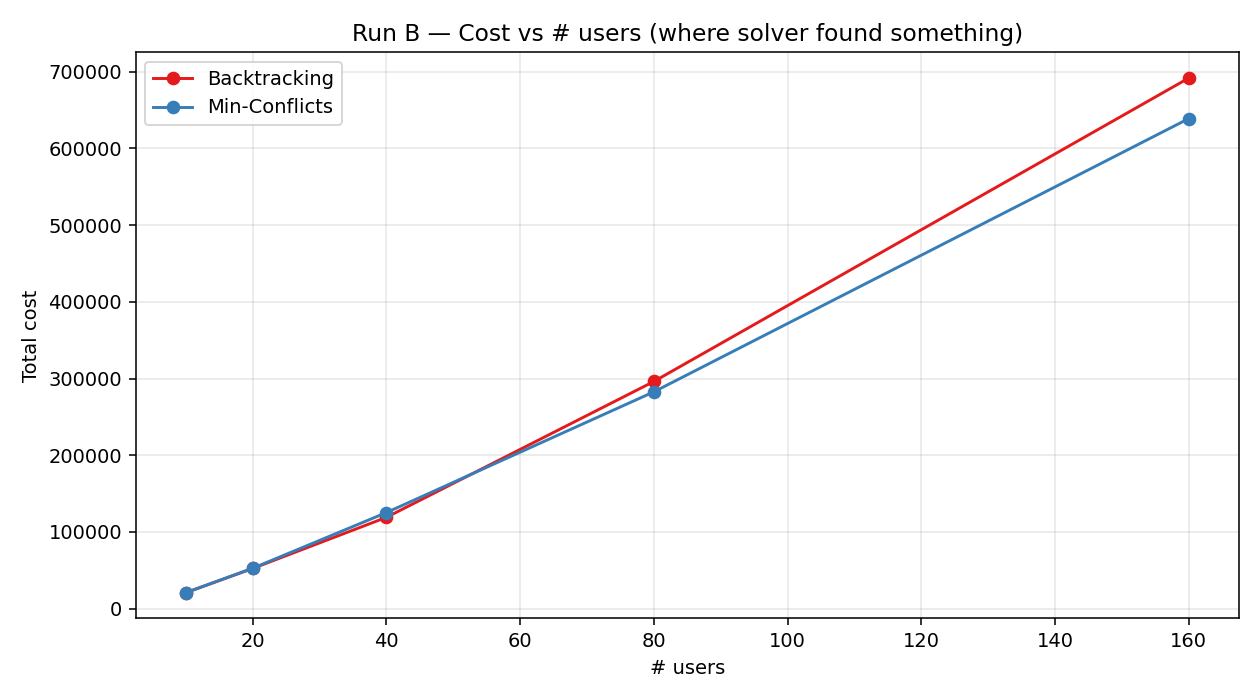
\includegraphics[width=\linewidth]{figures/a2_scaling_cost.png}
    \caption{Solution cost vs.\ $n$.}
  \end{subfigure}
  \caption{Scaling sweep: backtracking vs.\ Min-Conflicts as the number of users grows. Min-Conflicts is faster throughout while matching solution cost.}
  \label{fig:a2scaling}
\end{figure}

\paragraph{Study~C   Policy Validation under Aggressive Rationing.}
The aggressive rationing policy restricts feasibility rather than solver behavior. On a realistic city-scale instance of $150$ users and $30$ stations, only $32$ users are servable, leaving $118$ unassignable. This is not a solver failure, but a policy constraint: plate-parity wipe-outs, emergency reserves, CNG closures, and capacity limits empty user domains before search begins. \Cref{fig:a2full} (right) visualizes this sparse city-wide assignment. The CSP framework thus acts as a policy validator, proving that severe rationing cannot achieve full service coverage.

\begin{figure}[H]
  \centering
  \begin{subfigure}{0.49\linewidth}
    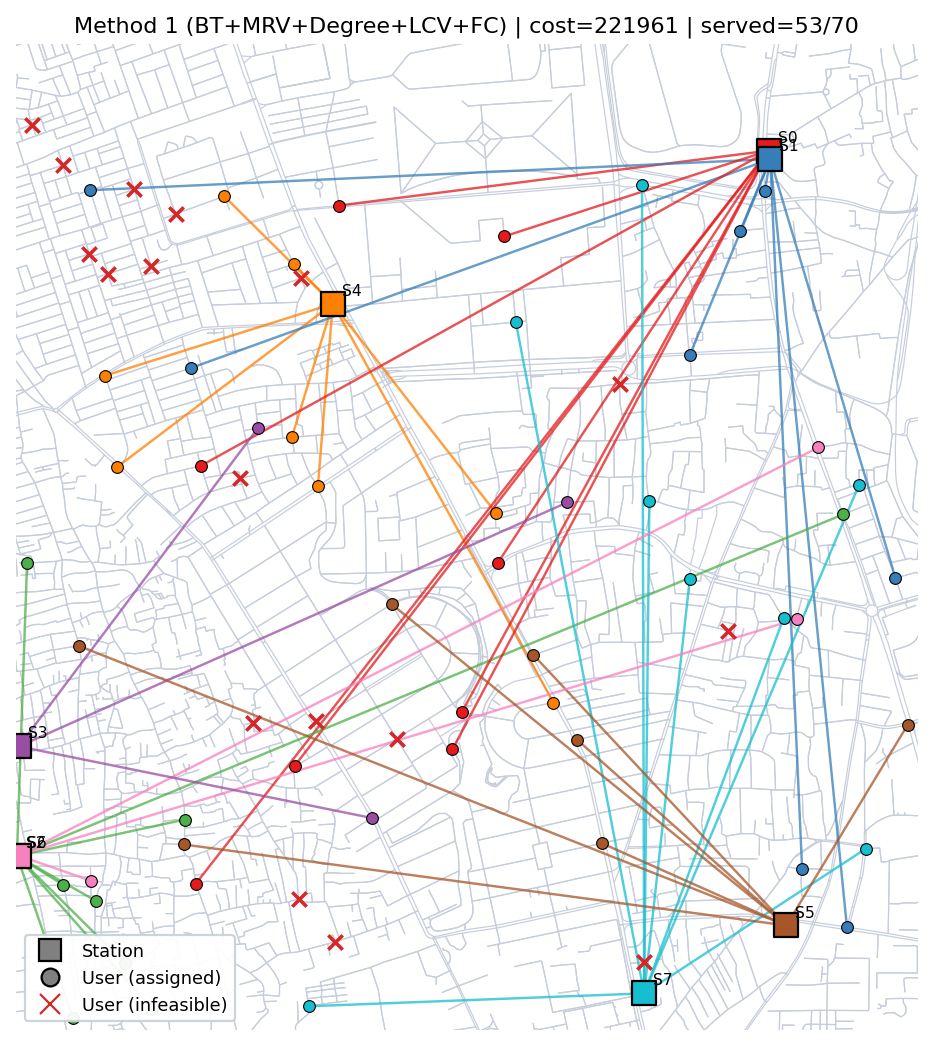
\includegraphics[width=\linewidth]{figures/a2_bt_map.png}
    \caption{Worked example: $12$ users, $8$ stations (Dhanmondi).}
  \end{subfigure}\hfill
  \begin{subfigure}{0.49\linewidth}
    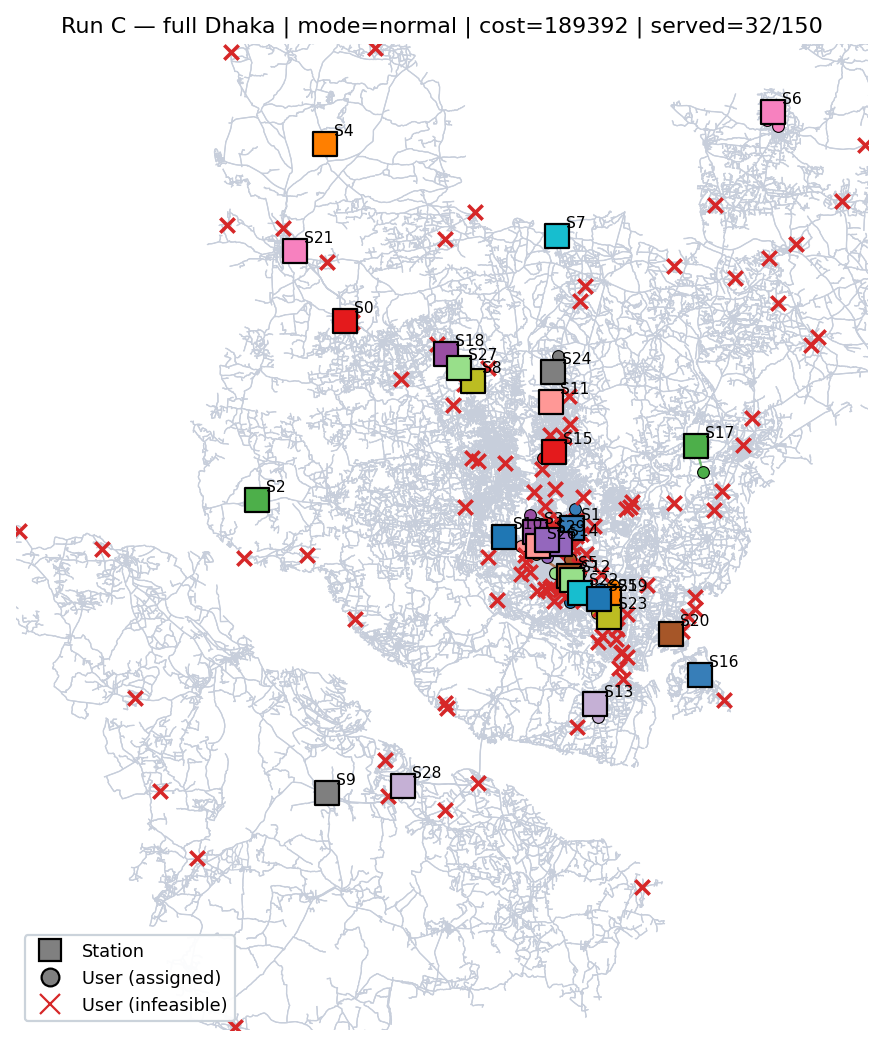
\includegraphics[width=\linewidth]{figures/a2_full_map.png}
    \caption{Full-Dhaka assignment (150 users, 30 stations).}
  \end{subfigure}
  \caption{Color-coded user-to-station assignments on real Dhaka roads at two scales: a small worked example (left) and the full city (right), where aggressive rationing leaves $118/150$ users unassignable  a feasibility limit of the policy, not a solver failure.}
  \label{fig:a2}\label{fig:a2full}
\end{figure}


\subsection{Key Takeaways and Empirical Synthesis}
\label{sec:a2takeaways}

Our evaluation of the CSOP framework for urban fuel rationing yields three primary insights:

\begin{enumerate}
  \item \textbf{Heuristic Pruning Eliminates Combinatorial Explosion}: AC-3 arc consistency, MRV variable ordering, and forward checking turn intractable depth-first backtracking into an instant solver for feasible instances ($n\le70$, 0 backtracks). On infeasible instances, however, ordering heuristics add per-node overhead without reducing backtracks, revealing that lookahead accelerates \emph{finding} solutions rather than \emph{proving} inconsistency.
  \item \textbf{Systematic vs.\ Local Search Scalability}: Systematic backtracking hits an absolute combinatorial wall between $n=70$ and $n=100$ ($>150{,}000$ backtracks, timing out). In contrast, Min-Conflicts local search scales smoothly up to $n=160$ ($2.60$\,ms runtime), directly optimizing the soft load-balancing cost \cref{eq:cspcost} while sacrificing completeness guarantees.
  \item \textbf{Rationing Feasibility Bounds}: On a full city-scale instance ($150$ users, $30$ stations), strict plate-parity, emergency reserves, and queue caps render $118$ users unassignable due to domain wipe-outs before search even commences. The CSP framework thus acts as a formal policy validator, proving that severe supply rationing cannot achieve full service coverage.
\end{enumerate}

While this CSOP addresses static, discrete multi-user assignment under hard policy constraints, urban services often require 
continuous spatial placement under non-submodular objectives or dynamic adaptive policies. In \Cref{sec:a3}, we transition 
to population-based optimization (CCTV camera placement).

% =====================================================================
\section{Population-Based Optimization for Surveillance-Camera Placement}
\label{sec:a3}\label{sec:swarm}

\subsection{Problem Formulation}
\label{subsec:a3cctv}

Public-safety surveillance is a resource-allocation problem under a hard budget: a city can afford only a fixed number of cameras, yet must watch the roads and public spaces where incidents are most likely and most costly. Dhaka makes this concrete. The Dhaka Metropolitan Police is rolling out a city-wide municipal CCTV network and integrating a large number of private cameras into a central monitoring grid, and densely monitored zones such as Gulshan--Baridhara are reported to experience lower crime than sparsely covered areas~\citep{tbs2023cctv,dailystar2023cctv}. Unlike blanket coverage, a real deployment must decide not only \emph{where} to mount each unit but \emph{which way it faces}, since a camera sees only a directional cone. The planning question we study is therefore: \emph{given a limited camera budget, where and facing which direction should each camera be placed to watch the most important and highest-risk roads?} We formalize this as a directional Maximal Covering Location Problem (MCLP), which is NP-hard~\citep{church1974maximal}.

\textbf{Inputs.} A Dhaka neighbourhood road graph; a demand field of weighted points $p$ (road samples weighted by road importance, junctions by degree, boosted near real OSM points-of-interest, and modulated by a crime/crowd risk field); a fixed camera budget $K$; and a fleet of directional cameras, each with a field-of-view angle FOV and range $R$.

\textbf{Output.} A placement that assigns to each camera $k$ an intersection $n_k$ and a facing angle $\theta_k$ (the decision variables). A demand point $p$ is \emph{covered} iff it lies within some camera's range \emph{and} field-of-view cone.

\textbf{Objective.} Among placements, maximize weighted coverage, optionally penalizing redundant overlap:
\begin{equation}
\mathcal{F}(\{n_k,\theta_k\}) \;=\; \underbrace{\textstyle\sum_{p:\,c_p\ge1} w_p}_{\text{weighted coverage}} \;-\; \lambda\underbrace{\textstyle\sum_{p} w_p\,\max(0,\, c_p-1)}_{\text{overlap penalty}},
\label{eq:cctvobj}
\end{equation}
where $c_p$ is the number of cameras that see point $p$, $w_p$ its weight, and $\lambda$ the overlap penalty. With $\lambda=0$ the objective is \emph{submodular} (plain coverage); with $\lambda>0$ redundant coverage is penalized and the objective becomes \emph{non-submodular} a distinction that turns out to decide which algorithm wins. \Cref{tab:a3notation} collects the notation.

\begin{table}[H]
\centering
\small
\begin{tabularx}{\linewidth}{@{}lX@{}}
\toprule
Symbol & Meaning \\
\midrule
$K$ & camera budget (number of cameras to place) \\
$R,\ \text{FOV}$ & camera range and field-of-view angle \\
$(n_k,\theta_k)$ & intersection and facing angle of camera $k$ (the decision variables) \\
$w_p$ & weight of demand point $p$ = road importance $\times$ POI $\times$ crime factor \\
$c_p$ & number of cameras covering $p$ \\
$\lambda$ & overlap penalty ($0$ = submodular; $>0$ = non-submodular) \\
\bottomrule
\end{tabularx}
\caption{Assignment~3 notation. Numeric settings for every symbol are justified in \Cref{sec:a3defend}.}
\label{tab:a3notation}
\end{table}

We treat this study as a controlled empirical comparison of three population-based optimizers against a greedy baseline, analysed in \Cref{sec:a3aresults}, targeting three questions. First, on a \emph{submodular} coverage objective ($\lambda{=}0$), whether the population-based methods (GA, PSO, ACO) improve on a greedy baseline. Second, when an overlap penalty makes the objective \emph{non-submodular} ($\lambda{>}0$), whether a metaheuristic overtakes greedy, and which mechanism is responsible. Third, whether the synthetic crime/crowd layer steers placement toward high-risk zones, and how coverage transfers across Dhaka neighbourhoods.

\subsection{Methodology}

\subsubsection{Simulation Environment and Demand Model}
A neighbourhood sub-graph is cropped from the Dhaka OSM graph obtained through OSMnx~\citep{boeing2017osmnx}. Road segments are sampled into \emph{demand points}, each weighted by three multiplicative factors: the OSM importance of the road it lies on (arterials outrank service lanes), the degree of the nearest intersection (busy junctions outrank dead-ends), and a proximity boost for points near real OSM points-of-interest (schools, markets, hospitals, bus stands). A synthetic \emph{crime/crowd risk field} a sum of Gaussian ``risk'' clusters, part of them seeded on real POIs and the rest placed pseudo-randomly, fully determined by the run seed further multiplies the weights so that placement is pulled toward high-risk zones. Camera coverage is modelled as a directional cone: a point $p$ is covered by camera $k$ iff the Euclidean line-of-sight distance $\lVert p-n_k\rVert\le R$ \emph{and} the bearing of $p$ from $n_k$ lies within $\theta_k\pm\text{FOV}/2$. Line-of-sight (rather than road-network) distance is used here because a camera sees across open space, unlike a car in Assignments~1--2 which must follow the road graph.

\subsubsection{Design Rationale and Empirical Basis}
\label{sec:a3defend}

A coverage model is only as credible as the reasoning behind its terms, so we justify each numeric choice rather than merely assert it. Every value below is a design parameter of the simulated environment, not a fitted measurement.

\paragraph{(i) Demand weighting.} The multiplicative weight $w_p = (\text{road importance})\times(\text{junction degree})\times(\text{POI proximity})\times(\text{crime factor})$ encodes the real surveillance priority behind the DMP rollout: busy arterials, crowded junctions, and high-footfall public sites matter more than quiet residential lanes~\citep{tbs2023cctv,dailystar2023cctv}. Only the \emph{ordinal} structure is asserted an arterial junction near a market outweighs a back-street not the precise multipliers.

\paragraph{(ii) Crime/crowd risk field.} Because open, edge-level crime data for Dhaka is not publicly available at the required granularity, we \emph{synthesize} a risk field rather than fit one. It is a sum of Gaussian clusters (baseline: a handful of clusters, roughly half anchored on real POIs and half placed pseudo-randomly, each with a few-hundred-metre spread), deterministic per seed so every solver sees an identical instance. This mirrors the earlier assignments' stance: the field is a transparent stand-in whose \emph{shape} elevated risk around crowded hubs is what matters, not its absolute magnitudes.

\paragraph{(iii) Camera physics.} The fleet mixes two sensor types whose reach reflects commodity CCTV optics: wide-angle $90^\circ$ units with a $200$\,m effective range, and narrower $120^\circ$ units with a $130$\,m range (a wider cone trades range for breadth). These are the physical constants of the coverage cone; the range-sensitivity sweep of \Cref{sec:a3aresults} scales them explicitly to show the model responds as expected.

\paragraph{(iv) Budget and fleet.} The baseline budget is $K{=}15$ cameras for a typical neighbourhood, raised to $K{=}30$ for the dense adversarial regime. The fleet is a fixed mix of the two sensor types. Both are operational choices a planner sets from a procurement budget the model treats $K$ as a free knob and reports how coverage scales with it.

\paragraph{(v) Overlap penalty $\lambda$.} The penalty $\lambda$ in \cref{eq:cctvobj} is the single lever that converts a pure (submodular) coverage objective into a redundancy-averse (non-submodular) one. We treat it as the primary experimental control and sweep it over a range from $0$ (plain coverage) up to values large enough that avoiding double-coverage dominates, precisely to locate where a metaheuristic starts to matter.

\paragraph{(vi) Optimizer representation and controls.} The three population-based optimizers differ along three deliberate axes how they represent the facing angle $\theta$, their search operators, and the controls they share summarized in \Cref{tab:a3hyper}. Two controls are common to all three: a \emph{memetic warm start}~\citep{neri2012memetic} (one individual / particle / ant path is seeded with the greedy baseline layout,\footnote{The greedy baseline is not one of the population methods under study; it builds a layout one camera at a time, each time adding the (node, one-of-$16$-directions) camera of largest marginal gain in $\mathcal F$, using $16$ fixed directions and one camera per node. It is fast and, on a submodular objective, near-optimal by the classic $(1-1/e)$ guarantee, so we use it as a strong starting point and comparison baseline.} so no metaheuristic can score below greedy), and \emph{early stopping} with a patience of $20$ under a cap of $200$ iterations ($500$ in the adversarial study). The single decisive representation choice is the facing angle: only PSO carries $\theta$ as a \emph{continuous} variable, whereas ACO samples $8$ fixed angle bins and GA mutates $\theta$ in discrete jumps the crux of why PSO alone can trim the fine overlap that a penalty punishes.

\begin{table}[H]
\centering
\small
\begin{tabularx}{\linewidth}{@{}llXX@{}}
\toprule
Optimizer & Angle $\theta$ & Representation & Key hyper-parameters \\
\midrule
GA & discrete jumps & $K$ genes $(node,\ \theta)$ & pop $40$, tournament $3$, crossover $0.85$ (uniform), mutation $0.2$ (move node / rotate $\theta{\sim}\mathcal N(0,0.6)$), elitism $2$ \\
PSO & \textbf{continuous} & continuous $(x,y,\theta)^{K}$, snapped to nearest node & swarm $30$, inertia $w{=}0.7$, cognitive $c_1{=}1.5$, social $c_2{=}1.5$ \\
ACO & $8$ fixed bins & subset of $K$ nodes $+$ angle bin & ants $20$, $\alpha{=}1$ (pheromone), $\beta{=}2$ (heuristic $\eta$), evaporation $\rho{=}0.1$, elitist deposit \\
\bottomrule
\end{tabularx}
\caption{Per-optimizer representation and hyper-parameters (identical across all runs; tunable design settings, not fitted values). All three are warm-started from the greedy baseline.}
\label{tab:a3hyper}
\end{table}

\emph{On the simulation framing.} This environment is explicitly a \emph{simulation}: none of the demand weights, crime clusters, camera ranges, or solver hyper-parameters is a measured Dhaka quantity, and each can be replaced by a calibrated real-data estimate without touching the optimization or evaluation code. The framework is fully modular, and every empirical claim we make depends only on \emph{relative} solver behaviour which method wins, and under what objective structure not on the absolute value of any single constant.

\subsubsection{From Coverage Model to Optimization: The Algorithmic Approach}

Before detailing each optimizer, it is worth being precise about \emph{how} the coverage objective connects to the search machinery because one representation choice in particular is exactly what separates the three methods.

\paragraph{What every optimizer receives.}
All three optimizers operate on the same instance and call the same objective $\mathcal F(\{n_k,\theta_k\})$ from \cref{eq:cctvobj} to score any complete $K$-camera layout. None of them has gradient access; $\mathcal F$ is a black box evaluated by counting which weighted demand points fall inside which cones. Each is \emph{warm-started} from the greedy baseline layout (\Cref{sec:a3defend}), so each begins from an already-strong solution it can only improve on. What they do \emph{not} share is how they represent the facing angle $\theta$ (\Cref{tab:a3hyper}), and as the three descriptions below make clear that single difference is the whole story.

\paragraph{Genetic Algorithm.}
The GA~\citep{holland1975adaptation} evolves a population of $K$-gene chromosomes (\Cref{alg:a3ga}). Tournament selection, uniform crossover, and mutation (move a camera to another node, or rotate its angle) explore combinations the baseline never considers but because its angle mutations are \emph{discrete jumps}, it cannot finely tune a facing direction.

\begin{algorithm}[H]
\caption{Genetic Algorithm (chromosome $=$ $K$ genes, each a $(node,\theta)$ pair).}
\label{alg:a3ga}
\begin{algorithmic}[1]
\State population $P\gets$ random $K$-camera layouts, one seeded with the greedy layout
\For{generation $=1,2,\dots$ (until stagnation)}
  \State evaluate fitness $\mathcal F$ \cref{eq:cctvobj} of every layout;\ keep the top $e$ (elitism)
  \While{$P$ not refilled}
    \State $p_1,p_2\gets$ tournament-select;\ \ child $\gets$ uniform crossover of $p_1,p_2$
    \State mutate: move a camera to a random node \emph{or} rotate its $\theta$;\ repair one-per-node
  \EndWhile
\EndFor
\State \Return best layout
\end{algorithmic}
\end{algorithm}

\paragraph{Particle Swarm Optimization.}
PSO~\citep{kennedy1995pso} treats a layout as a point in continuous $(x,y,\theta)^K$ space (\Cref{alg:a3pso}). Each particle is pulled toward its own and the swarm's best positions; the $(x,y)$ coordinates snap to the nearest intersection, but the angle $\theta$ stays \emph{continuous}. This is the one optimizer that can dial a facing direction to any value the property that lets it trim overlap the discrete methods cannot.

\begin{algorithm}[H]
\caption{Particle Swarm Optimization (particle $=$ continuous $(x,y,\theta)^{K}$, snapped to nearest node).}
\label{alg:a3pso}
\begin{algorithmic}[1]
\State initialize positions $x_i$, velocities $v_i$; seed one particle with greedy; set $pbest_i,gbest$
\For{iteration $=1,2,\dots$ (until stagnation)}
  \ForAll{particle $i$}
    \State $v_i\gets w\,v_i+c_1 r_1(pbest_i-x_i)+c_2 r_2(gbest-x_i)$;\ \ $x_i\gets\operatorname{clip}(x_i+v_i)$
    \State decode: snap each $(x,y)$ to its nearest intersection;\ evaluate $\mathcal F$
    \State update $pbest_i$ and $gbest$
  \EndFor
\EndFor
\State \Return $gbest$
\end{algorithmic}
\end{algorithm}

\paragraph{Ant Colony Optimization.}
ACO~\citep{dorigo1996antsystem} builds layouts by sampling $K$ distinct nodes with probability $\propto\tau^\alpha\eta^\beta$ (pheromone $\times$ single-camera desirability), then an angle bin per node (\Cref{alg:a3aco}). Pheromone reinforces good regions across iterations, but its angles are drawn from $8$ fixed bins again discrete.

\begin{algorithm}[H]
\caption{Ant Colony Optimization (subset selection of $K$ intersections $+$ discrete angles).}
\label{alg:a3aco}
\begin{algorithmic}[1]
\State pheromones $\tau_{\text{node}},\tau_{\text{ang}}\gets1$; heuristic $\eta_c=$ best single-camera coverage of node $c$; seed best from greedy
\For{iteration $=1,2,\dots$ (until stagnation)}
  \ForAll{ant}
    \State build a layout: pick $K$ distinct nodes with prob.\ $\propto\tau_{\text{node}}^{\alpha}\eta^{\beta}$, and an angle bin per node
    \State evaluate $\mathcal F$
  \EndFor
  \State evaporate $\tau\gets(1-\rho)\tau$;\ \ deposit $\propto\mathcal F$ on the best-so-far layout (elitist)
\EndFor
\State \Return best layout
\end{algorithmic}
\end{algorithm}

\paragraph{The greedy baseline.}
For reference, the three optimizers are all measured against a simple greedy baseline (used above only as their warm-start seed, not as a method under study). It builds a layout one camera at a time, each step adding the (node, one-of-$16$-directions) camera of largest marginal gain in $\mathcal F$ and never revisiting an earlier choice. On a submodular objective this myopia is nearly harmless the classic $(1-1/e)$ guarantee makes it near-optimal but once it clusters cameras at the busiest hub it cannot undo the resulting redundancy, which is precisely the weakness the penalized regime exposes.

When $\lambda=0$ the objective is submodular and the greedy baseline is already near-optimal, so warm-started metaheuristics can only tie it adding search machinery buys nothing. The moment $\lambda>0$ makes the objective non-submodular, redundant overlap must be actively trimmed, and trimming it well requires \emph{fine} control of the facing angle. Only PSO's continuous $\theta$ provides that, which predicts that PSO and \emph{only} PSO should overtake greedy in the penalized regime. This is the central empirical question of the assignment, and \Cref{sec:a3aresults} tests it directly.

\subsubsection{Evaluation Metrics and Experimental Protocol}
Our study demonstrates,
\begin{itemize}[leftmargin=1.4em,itemsep=2pt,topsep=2pt]
  \item \textbf{Weighted coverage (\%)}   the fraction of total demand weight seen by at least one camera; the primary quality measure.
  \item \textbf{Overlap (\%)}   the weight counted redundantly ($c_p\ge2$); the quantity the penalty $\lambda$ targets.
  \item \textbf{Objective}   the penalized score $\mathcal F$ of \cref{eq:cctvobj} that the solvers actually maximize.
  \item \textbf{Runtime}   wall-clock seconds to converge.
  \item \textbf{Iterations}   generations / swarm steps / ant rounds until early stopping.
\end{itemize}

Controlled sweeps vary one factor at a time while holding the graph, fleet, and solver settings fixed: the crime layer on/off, the camera budget $K$, the camera range, the neighbourhood, and critically the overlap penalty $\lambda$. To expose greedy's myopia decisively, we add a deliberately adversarial ``greedy-fail'' scenario: a tiny $500$\,m area packed with $30$ very-long-range cameras, where a single camera already covers a large share of demand, so avoiding redundant overlap is the entire game. The overall workflow is summarized in \Cref{fig:a3workflow}.

\begin{figure}[H]
  \centering
  \begin{tikzpicture}[
    node distance=1.5cm and 0.55cm,
    every node/.style={draw, rounded corners, align=center,
      minimum width=2.05cm, minimum height=0.7cm, fill=blue!5, font=\small},
    >=Latex]
    \node (g) {OSM\\neighbourhood};
    \node (d) [right=of g] {Weighted demand\\(+ crime field)};
    \node (gr) [right=of d] {Greedy\\seed};
    \node (op) [right=of gr] {Optimizers\\(GA/PSO/ACO)};
    \node (o) [right=of op] {Layout\\+ coverage};
    \draw[->,thick] (g) -- (d);
    \draw[->,thick] (d) -- (gr);
    \draw[->,thick] (gr) -- (op);
    \draw[->,thick] (op) -- (o);
  \end{tikzpicture}
  \caption{Workflow: a weighted, crime-aware demand field defines the coverage objective; a greedy layout seeds the metaheuristics, which refine node placement and facing angles.}
  \label{fig:a3workflow}
\end{figure}

\subsection{Results and Discussion}
\label{sec:a3aresults}

\paragraph{Worked test case}
\mbox{}\\
\textbf{Scenario.} 
Before the aggregate sweeps, we walk through one concrete instance: place $K{=}15$ cameras in Dhanmondi with the crime/crowd layer enabled and no overlap penalty ($\lambda{=}0$). The greedy baseline first builds a layout by repeatedly adding the camera of largest marginal coverage gain; each optimizer is warm-started from that layout and is then free to move nodes and rotate facing angles.

The chosen cameras concentrate on the high-risk red zones of the crime field (\Cref{fig:a3}, left) rather than spreading uniformly, and the PSO solution's field-of-view wedges tile the busy arterials and junctions of the real Dhanmondi road graph (right). Turning the crime layer on lifts weighted coverage from $21.9\%$ to $25.3\%$ as cameras migrate toward risk direct evidence that the weighted-demand model steers placement where a real deployment would want it. On this submodular instance all three optimizers converge to exactly the same $25.3\%$ as the greedy seed: none can improve on an already near-optimal baseline. Whether that tie is fundamental or an artefact of this easy regime is what the aggregate sweeps below resolve.

\begin{figure}[H]
  \centering
  \begin{subfigure}{0.48\linewidth}
    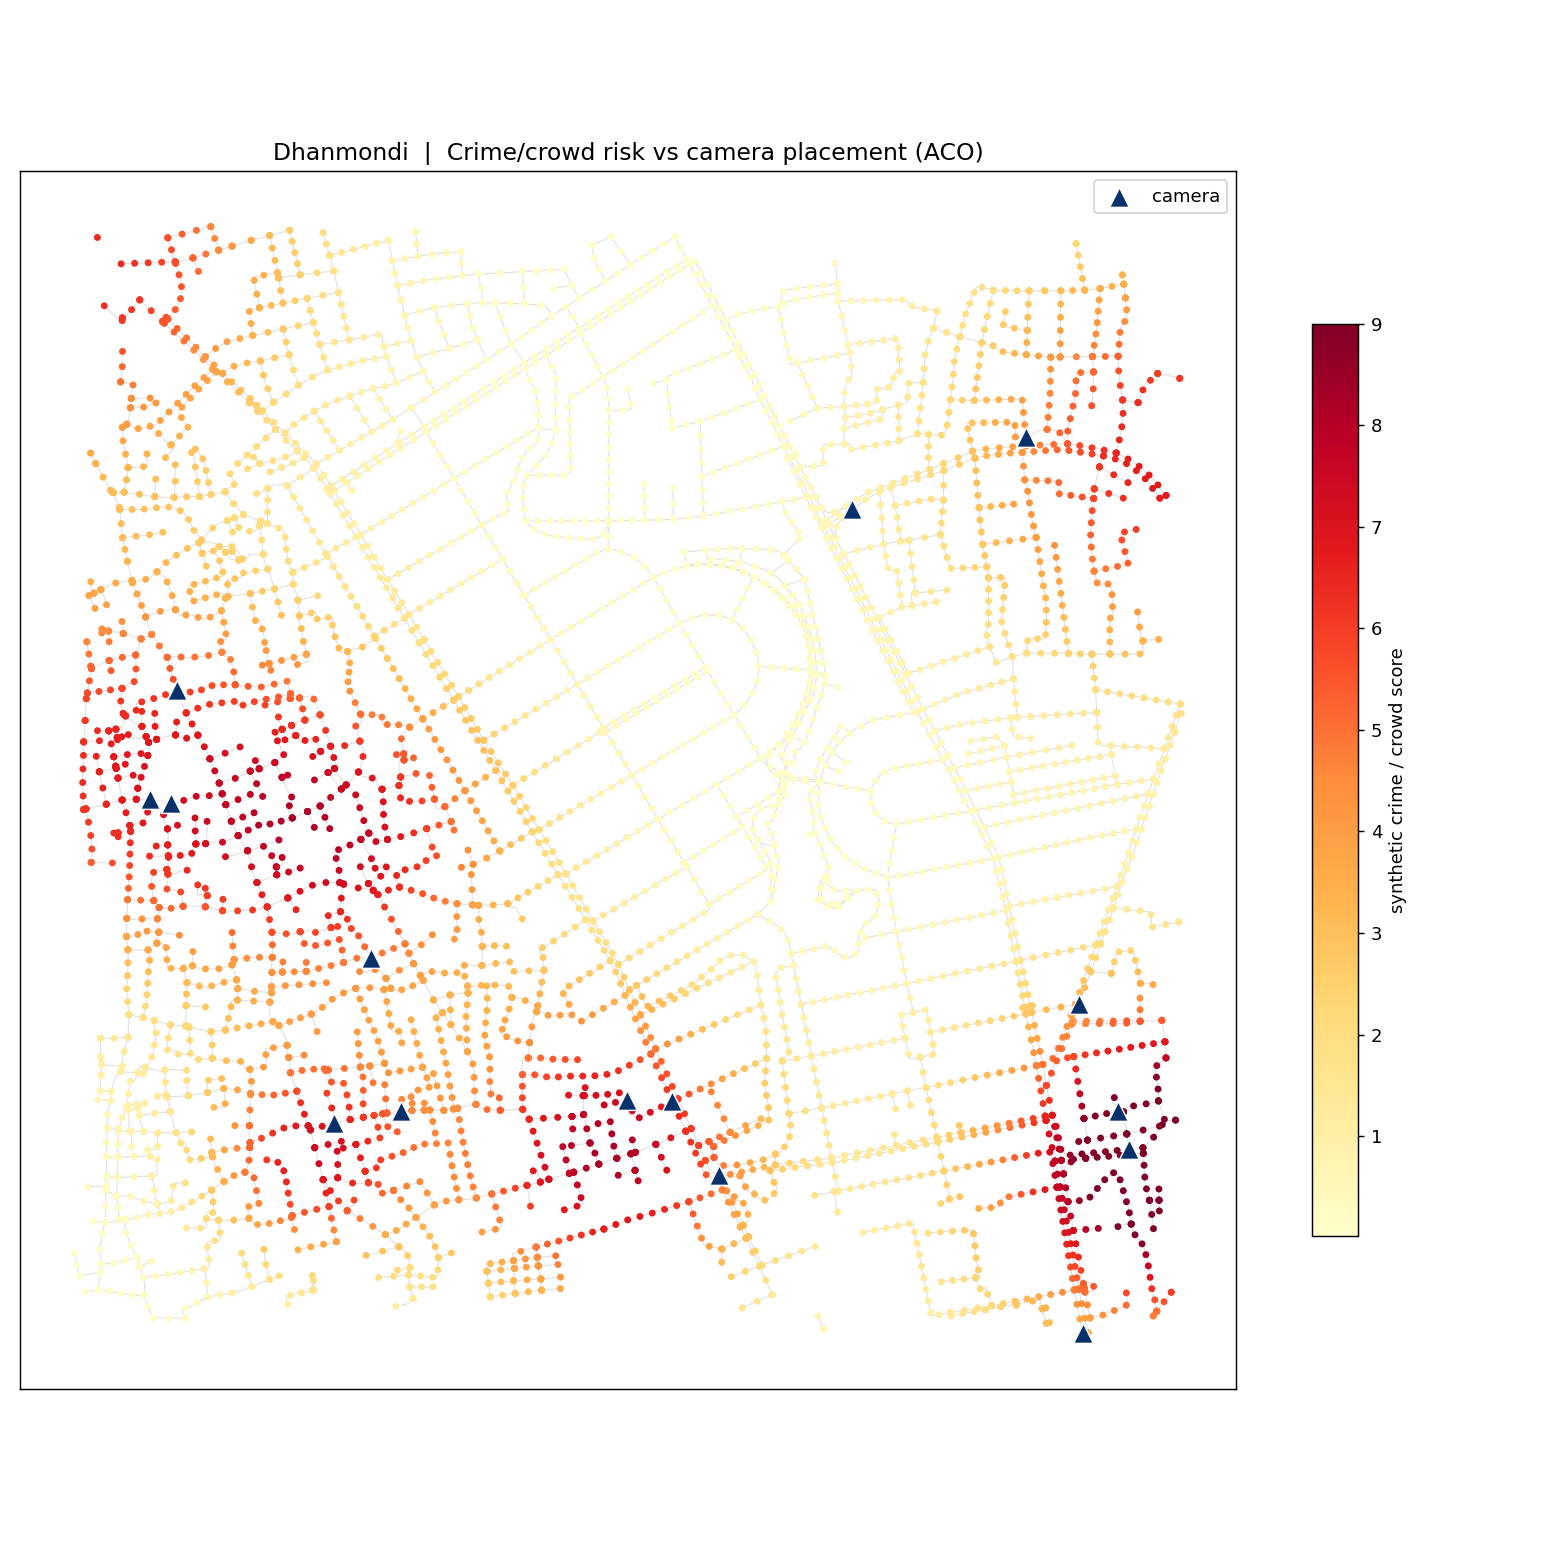
\includegraphics[width=\linewidth]{figures/a3_crime_heatmap.png}
    \caption{Crime/crowd risk field with chosen cameras.}
  \end{subfigure}\hfill
  \begin{subfigure}{0.48\linewidth}
    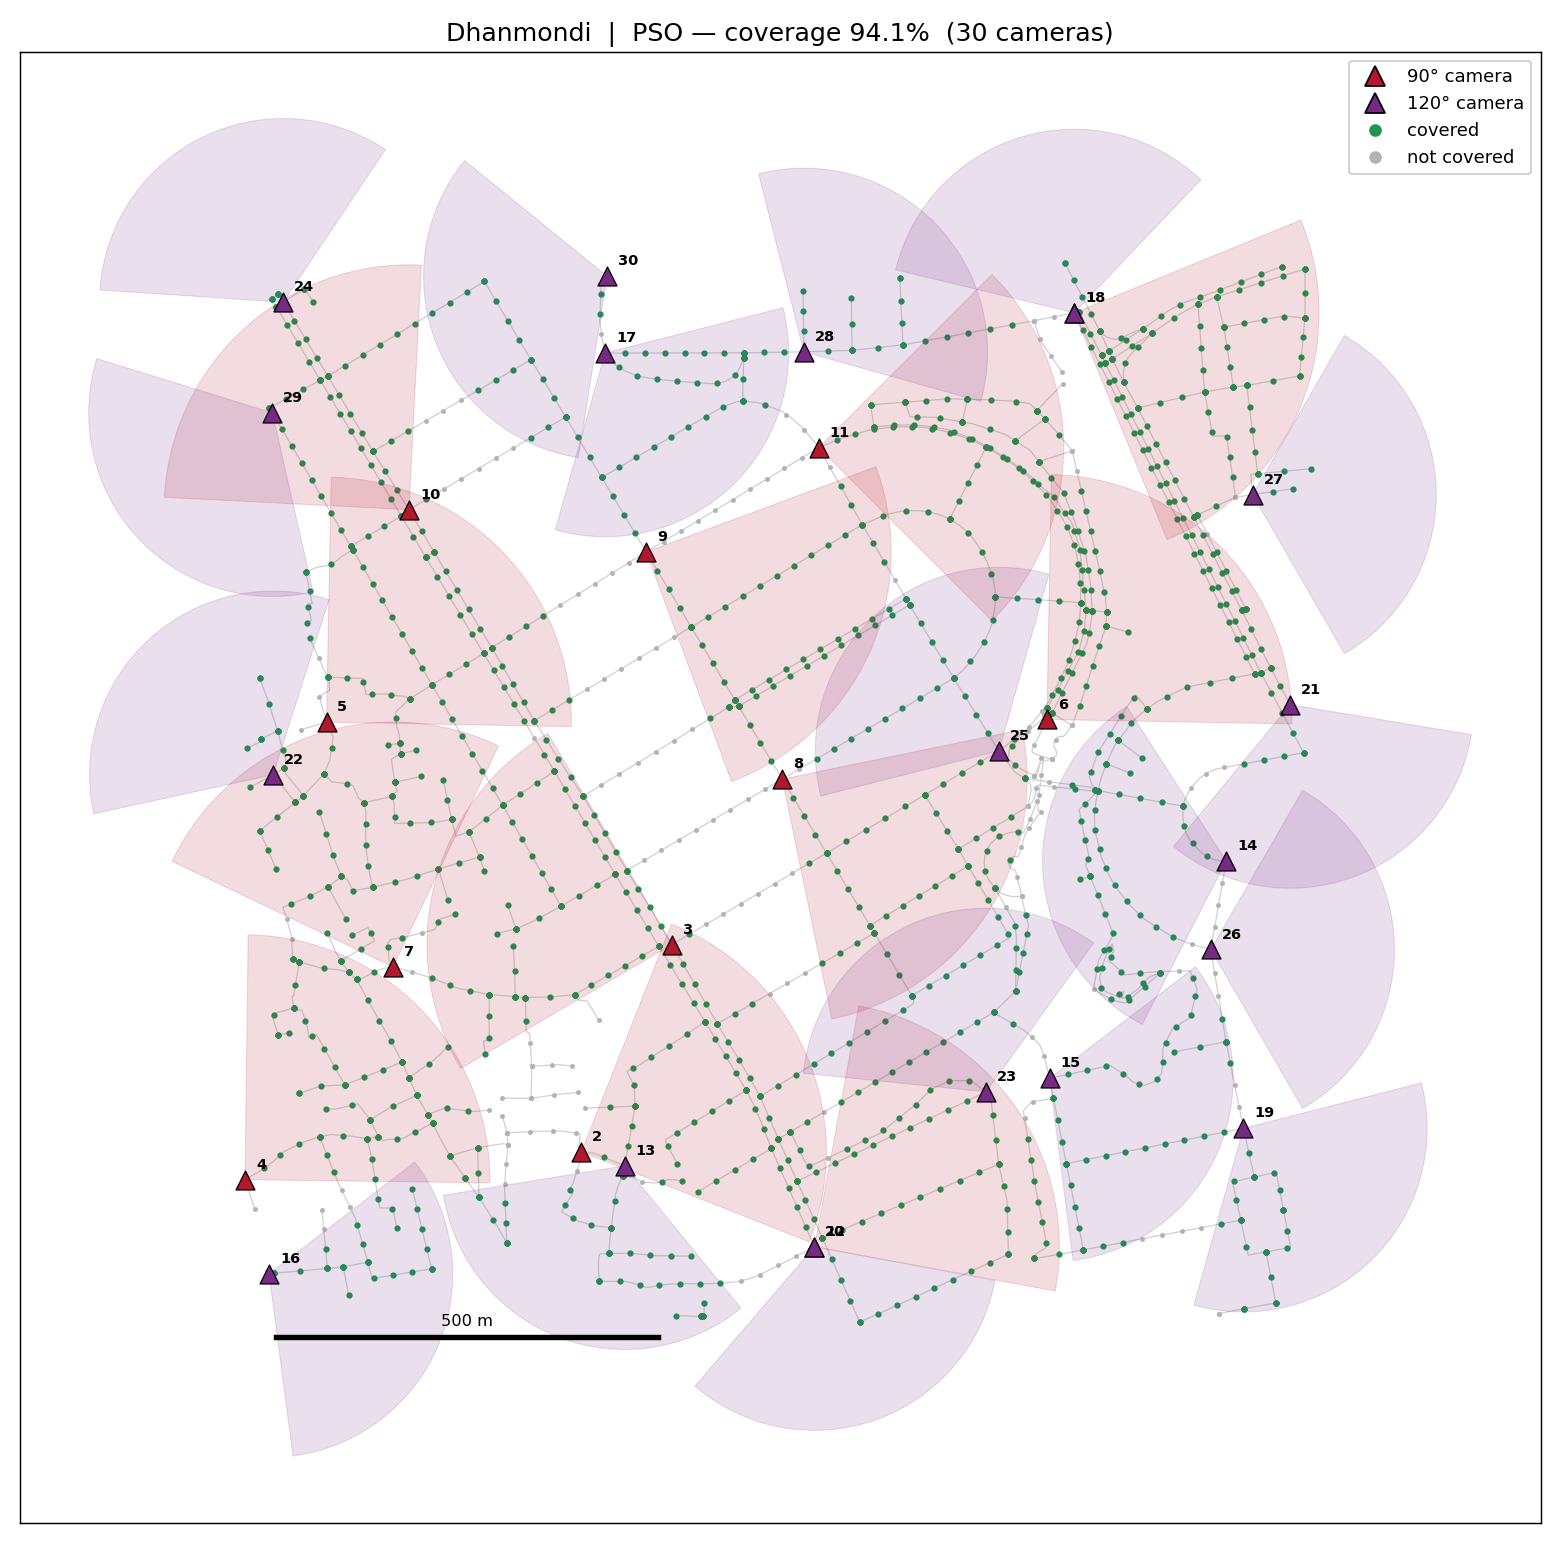
\includegraphics[width=\linewidth]{figures/a3_pso_map.png}
    \caption{PSO placement with field-of-view wedges.}
  \end{subfigure}
  \caption{Worked test case (Dhanmondi, $K{=}15$, crime layer on): cameras concentrate in high-risk red zones (left); the PSO solution and its coverage cones on real Dhaka roads (right).}
  \label{fig:a3}
\end{figure}

\paragraph{Aggregate Analysis}
\mbox{}\\
 We now generalize from this single instance to controlled multi-scenario sweeps covering three regimes: the submodular baseline, the non-submodular penalty regime, and crime steering with neighbourhood transfer.

For plain coverage ($\lambda=0$, $K=15$) all three optimizers tie the greedy baseline at $\approx25.3\%$ weighted coverage (\Cref{tab:a3baseline}). This is expected: coverage is submodular, and greedy enjoys the classic $(1-1/e)\approx63\%$ optimality guarantee, so the warm-started metaheuristics can only match it. A metaheuristic is \emph{not} automatically better an honest and important baseline.

\begin{table}[H]
\centering
\small
\begin{tabularx}{\linewidth}{@{}Xrrr@{}}
\toprule
Metric & GA & PSO & ACO \\
\midrule
Weighted coverage (\%) & $25.3$ & $25.3$ & $25.3$ \\
\bottomrule
\end{tabularx}
\caption{Baseline (Dhanmondi, $K{=}15$, $\lambda{=}0$): all three optimizers tie the greedy baseline ($25.3\%$) on submodular coverage.}
\label{tab:a3baseline}
\end{table}

\paragraph{PSO overtakes greedy.}
Once an overlap penalty makes the objective non-submodular (dense scenario, $K=30$, long range), PSO \emph{consistently} exceeds greedy at every penalty level (\Cref{tab:a3cctv}), while GA and ACO whose angle moves are discrete only match it. The mechanism is specific: PSO optimizes the \emph{continuous} facing angle $\theta$, which greedy and the discrete methods can only sample in fixed steps, so PSO trims the redundant overlap they cannot. To expose this decisively we designed an adversarial ``greedy-fail'' scenario a tiny $500$\,m area packed with $30$ very-long-range cameras, where a single camera already covers ${\sim}40\%$ (\Cref{tab:a3greedyfail}). Here greedy's myopia is fatal: it commits cameras to the highest-demand hub and cannot undo the resulting redundancy, so its \emph{overlap stays stuck at ${\sim}4.5\%$}; PSO spreads the cameras out, cutting overlap below $1.5\%$ and beating greedy on coverage at every penalty. This is the clearest evidence that a metaheuristic genuinely outperforms greedy once the objective punishes redundancy the myopic baseline cannot escape mirroring Assignment~2's ablation lesson that the advanced method wins only when the problem \emph{structure} defeats the baseline's guarantee. \Cref{fig:a3compare} shows the solver comparison and convergence.

\begin{table}[H]
\centering
\small
\begin{tabularx}{\linewidth}{@{}Xrrrr@{}}
\toprule
$\lambda$ & Greedy & GA & PSO & ACO \\
\midrule
$0.0$ & $98.01$ & $98.01$ & $\mathbf{98.56}$ & $98.01$ \\
$0.5$ & $96.40$ & $96.40$ & $\mathbf{97.24}$ & $96.40$ \\
$1.0$ & $94.71$ & $94.71$ & $\mathbf{95.55}$ & $94.71$ \\
$2.0$ & $93.04$ & $93.04$ & $\mathbf{94.06}$ & $93.04$ \\
\bottomrule
\end{tabularx}
\caption{Dense, non-submodular regime ($K{=}30$): weighted coverage (\%). PSO beats greedy at every overlap penalty $\lambda$; GA and ACO (discrete angles) only match greedy.}
\label{tab:a3cctv}
\end{table}

\begin{table}[H]
\centering
\small
\begin{tabularx}{\linewidth}{@{}Xrrrr@{}}
\toprule
 & \multicolumn{2}{c}{Greedy} & \multicolumn{2}{c}{PSO (winner)} \\
\cmidrule(lr){2-3}\cmidrule(lr){4-5}
$\lambda$ & coverage \% & overlap \% & coverage \% & overlap \% \\
\midrule
$5$  & $90.6$ & $4.5$ & $\mathbf{93.6}$ & $1.5$ \\
$10$ & $90.6$ & $4.5$ & $\mathbf{91.9}$ & $0.8$ \\
$20$ & $92.8$ & $4.4$ & $\mathbf{93.0}$ & $1.0$ \\
\bottomrule
\end{tabularx}
\caption{Adversarial ``greedy-fail'' scenario ($500$\,m area, $30$ long-range cameras): coverage \emph{and overlap}. Greedy stays clustered at the busiest hub with ${\sim}4.5\%$ wasted overlap; PSO spreads cameras out, cutting overlap below $1.5\%$ and winning coverage at every penalty.}
\label{tab:a3greedyfail}
\end{table}

\begin{figure}[H]
  \centering
  \begin{subfigure}{0.48\linewidth}
    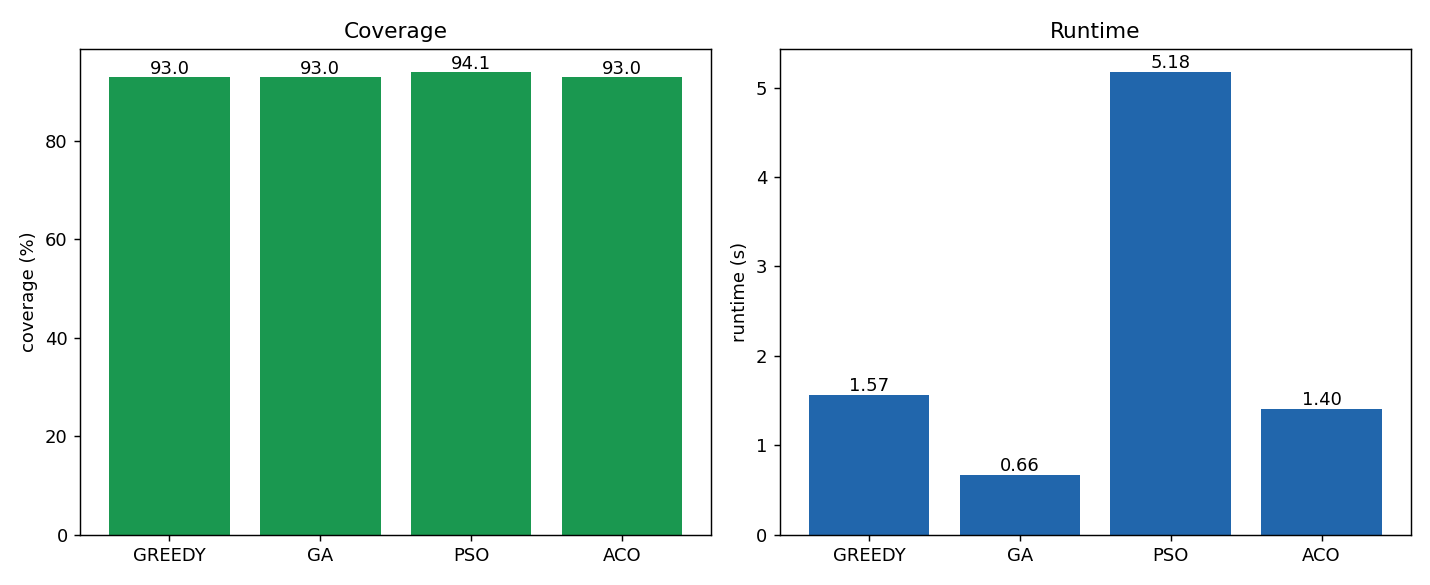
\includegraphics[width=\linewidth]{figures/a3_comparison.png}
    \caption{Coverage \& runtime by solver.}
  \end{subfigure}\hfill
  \begin{subfigure}{0.48\linewidth}
    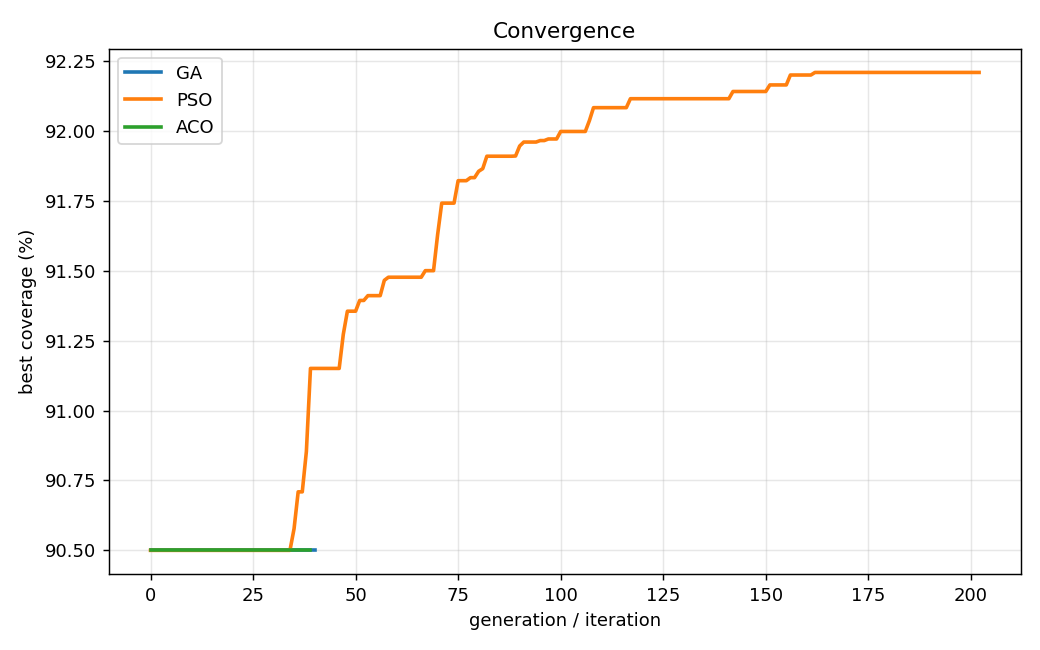
\includegraphics[width=\linewidth]{figures/a3_convergence.png}
    \caption{Convergence (coverage vs iteration).}
  \end{subfigure}
  \caption{Solver comparison (left) and convergence curves (right) in the dense non-submodular regime.}
  \label{fig:a3compare}
\end{figure}

\paragraph{Crime steering and neighbourhood transfer.}
The crime-steering effect quantified in the worked test case weighted coverage rising from $21.9\%$ to $25.3\%$ once the risk layer is enabled (\Cref{fig:a3}) holds across instances. Coverage also transfers sensibly across neighbourhoods (\Cref{tab:a3area}): Gulshan is easiest to cover ($36.3\%$) and Mirpur hardest ($24.1\%$). Reassuringly, this matches the real-world report that Gulshan's dense camera coverage coincides with lower crime~\citep{dailystar2023cctv} the model's easy-to-cover neighbourhood is the one that is, in practice, well covered.

\begin{table}[H]
\centering
\small
\begin{tabularx}{\linewidth}{@{}Xrrrrr@{}}
\toprule
Neighbourhood & Dhanmondi & Gulshan & Old Dhaka & Uttara & Mirpur \\
\midrule
Coverage (\%) & $25.3$ & $\mathbf{36.3}$ & $31.4$ & $30.1$ & $24.1$ \\
\bottomrule
\end{tabularx}
\caption{Neighbourhood transfer (weighted coverage \%, $K{=}15$).}
\label{tab:a3area}
\end{table}

\paragraph{Sensitivity to physical parameters.} Coverage is governed far more by the cameras' physical reach than by the choice of optimizer. Scaling the $90^\circ$ range from $140$ to $260$\,m lifts weighted coverage from $18.2\%$ to $32.9\%$, and because plain coverage is submodular all three optimizers return \emph{identical} values at each range (\Cref{tab:a3range}). Search budget shows the expected diminishing returns: PSO edges from $25.25\%$ at $20$ iterations to $25.48\%$ at $200$, while GA and ACO stay flat. The practical implication is that, in the submodular regime, longer-range (or more) cameras pay off more than a fancier optimizer the metaheuristic only earns its keep once the objective is non-submodular.

\begin{table}[H]
\centering
\small
\begin{tabularx}{\linewidth}{@{}Xrrr@{}}
\toprule
$90^\circ$ camera range (m) & $140$ & $200$ & $260$ \\
\midrule
Weighted coverage (\%) & $18.2$ & $25.3$ & $32.9$ \\
\bottomrule
\end{tabularx}
\caption{Sensitivity: weighted coverage (\%) vs.\ camera range (all three optimizers return identical values under submodular coverage).}
\label{tab:a3range}
\end{table}

\subsection{Key Takeaways and Empirical Synthesis}
This study shows precisely when population-based optimization is worth its cost. On submodular coverage, greedy already achieves near-optimal placement and the warm-started metaheuristics can only tie it an honest baseline that resists the temptation to declare a metaheuristic automatically superior. The swarm advantage emerges only when an overlap penalty makes the objective non-submodular \emph{and} a continuous decision variable (the facing angle) is available: there PSO's continuous search overtakes greedy while the discrete GA and ACO do not, and the adversarial greedy-fail scenario isolates the mechanism greedy's myopic overlap stays stuck while PSO spreads the cameras out. Finally, the weighted-demand model, including the synthetic crime field, steers placement toward the high-risk zones that real Dhaka deployments target, and coverage transfers sensibly across neighbourhoods. The overarching lesson mirrors Assignment~2's ablation finding: the advanced method earns its keep only when the problem's \emph{structure} defeats the baseline's guarantee.

\section{Reinforcement Learning for Stochastic Multi-Stop Delivery}
\label{subsec:a3rl}\label{sec:rl}

\subsection{Motivation and Problem Formulation}
\label{sec:a4formulation}

On-demand delivery is now woven into daily life in Dhaka food, parcels, and tiffin services dispatch riders across the city continuously yet the same two forces that dominate the earlier assignments make each trip uncertain: traffic congestion that collapses average travel speed to a crawl at peak~\citep{worldbank2018dhaka,dailystar2018congestion}, and monsoon waterlogging that can render residential streets impassable within minutes~\citep{dailystar2025waterlogging}. A rider dispatched with several drop-offs one of them urgent must decide, at every junction and under this uncertainty, which way to head so as to complete all deliveries at the least expected cost while serving the urgent order first. Unlike the deterministic routing of Assignment~1, the outcome of each action here is \emph{stochastic}, so the agent needs not a single path but a \emph{policy}: a mapping from situation to action. We formalize this as a Markov Decision Process (MDP) $(S,A,T,R,\gamma)$~\citep{sutton2018rl,bellman1957dynamic}.

\textbf{Inputs.} A Dhaka neighbourhood road graph with per-edge travel times; a set of $K$ delivery stops (some flagged urgent); and hazard labels marking a fraction of roads as jammed or flooded. The MDP components are:
\begin{itemize}
  \item \textbf{State} $s=(v,U)$: current node $v$ and the set $U\subseteq\mathcal T$ of not-yet-visited stops (an immutable \code{frozenset} for hashing). There are $|V|\cdot 2^{K}$ states, so $K$ is kept small to avoid state-space explosion.
  \item \textbf{Action} $a$: a neighbouring node to head toward.
  \item \textbf{Transition} $T(s,a,s')$: \emph{stochastic}, depending on road type a normal road usually reaches the intended node, while a jammed or flooded road may divert or stall the agent (values in \Cref{sec:a4defend}).
  \item \textbf{Reward} $R$: a per-move travel-time cost, a hazard penalty for a divert/stall, a delivery bonus for reaching a stop (larger if urgent), and a completion bonus when all stops are served (magnitudes in \Cref{sec:a4defend}).
  \item \textbf{Discount} $\gamma$: makes earlier rewards worth more, so urgency is encoded via reward magnitude and discounting rather than a state-expanding deadline.
\end{itemize}
\textbf{Output.} An optimal policy $\pi^\ast: S\to A$ that maximizes the expected discounted return:
\begin{equation}
\pi^\ast \;=\; \arg\max_{\pi}\; \mathbb{E}_{\pi}\!\left[\,\sum_{t=0}^{\infty} \gamma^{t}\, r_t\,\right],
\label{eq:mdpobj}
\end{equation}
where $r_t$ is the reward at step $t$ and the expectation is taken over the stochastic transitions $T$ under policy $\pi$. Executing $\pi^\ast$ yields a delivery route that serves the urgent stop first. \Cref{tab:a4notation} lists the notation.

\begin{table}[H]
\centering
\small
\begin{tabularx}{\linewidth}{@{}lX@{}}
\toprule
Symbol & Meaning \\
\midrule
$s=(v,U)$ & state: current node $v$, unvisited stops $U$ \\
$K=|\mathcal T|$ & number of delivery stops; state count $=|V|\cdot2^{K}$ \\
$T(s,a,s'),\ R,\ \gamma$ & transition, reward, discount factor \\
$u(s),\ Q(s,a)$ & state value (VI) and action value (Q-Learning) \\
$\pi^\ast$ & optimal policy (state $\mapsto$ action) \\
\bottomrule
\end{tabularx}
\caption{Assignment~4 notation. Numeric settings are justified in \Cref{sec:a4defend}.}
\label{tab:a4notation}
\end{table}

We treat this study as a controlled empirical comparison of model-based planning against model-free learning on one stochastic routing problem, analysed in \Cref{sec:a4results}, targeting three questions. 

First, whether \emph{model-free} Q-Learning recovers the \emph{model-based} Value-Iteration optimum, and at what computational cost. 

Second, how sensitive the policy is to the discount $\gamma$, and where Q-Learning becomes unstable. 

Third, whether reward magnitude plus discounting correctly encodes delivery \emph{urgency}, and how the number of stops and hazards affect the solution and its tractability.

\subsection{Methodology}

\subsubsection{Simulation Environment and Hazard Model}
A sub-graph is cropped from the Dhaka OSM graph~\citep{boeing2017osmnx}. Each directed edge is assigned a deterministic travel time from its physical length and a road-type speed. Two hazard types then make travel \emph{stochastic}: a fraction of primary/secondary roads are marked \emph{jam}, and a fraction of residential/tertiary roads are marked \emph{flood}, both seeded so every agent faces an identical instance. On a normal road the agent almost always reaches the node it heads for; on a jammed road it may be diverted to an unintended neighbour; on a flooded road it may stall in place and lose the move. These outcomes define the transition $T(s,a,s')$, and each unwanted outcome carries a penalty in $R$.

\subsubsection{Design Rationale and Empirical Basis}
\label{sec:a4defend}

The MDP is only as credible as the numbers behind its transitions and rewards, so we justify each rather than assert it. Every value is a design parameter of the simulated environment.

\emph{(i) Stochastic transitions.} Each road type carries its own reach probability, mirroring the two forces that actually make Dhaka travel uncertain. A \emph{normal} road almost always delivers the agent to its intended node ($0.95$, with a $0.05$ chance of slipping to a random neighbour). \emph{Traffic}: average speed collapses to ${\sim}7$\,km/h in peak congestion, so a jammed arterial (primary/secondary road) frequently diverts a driver off the intended turn~\citep{worldbank2018dhaka,dailystar2018congestion}  we model this as a $0.70$ reach / $0.30$ divert split. \emph{Waterlogging}: monsoon rain routinely submerges residential and low-lying streets until they are impassable, stranding vehicles~\citep{dailystar2025waterlogging}  we model a flooded road (residential/tertiary) as a $0.50$ reach / $0.50$ stall split. Assigning jams to arterials and floods to smaller, low-lying roads matches the reported pattern.

\emph{(ii) Reward magnitudes.} The reward structure asserts only an \emph{ordinal} priority: completing all deliveries dominates ($+1000$), reaching an individual stop is worth a solid bonus ($+200$, doubled to $+400$ when urgent), a divert or stall is mildly punished ($-50$), and every move costs its travel time. These magnitudes are chosen so that the terminal goal is worth pursuing through several hazardous moves, not calibrated to any currency.

\emph{(iii) Urgency without a deadline.} Encoding urgency as a \emph{larger reward} rather than a hard time deadline is a deliberate modelling choice: a deadline would add a time dimension to the state and multiply the state count, whereas a reward bonus keeps the space at $|V|\cdot2^{K}$ while still driving the policy to serve urgent stops first.

\emph{(iv) Discount and agent controls.} Both agents share the discount $\gamma=0.95$ (its effect is swept in \Cref{sec:a4results}). Value Iteration stops when the Bellman residual falls below $\epsilon(1{-}\gamma)/\gamma$; Q-Learning adds a learning rate $\alpha$, an $\epsilon$-greedy decay schedule, and a convergence test (mean reward stable over three windows of $100$ episodes) so it can early-stop rather than always exhausting its episode budget. \Cref{tab:a4hyper} collects the settings.

\begin{table}[H]
\centering
\small
\begin{tabularx}{\linewidth}{@{}lXX@{}}
\toprule
Agent & Knowledge & Hyper-parameters \\
\midrule
Value Iteration & model-based (knows $T,R$) & $\gamma{=}0.95$; stop threshold $\epsilon{=}1.0$ ($\delta<\epsilon(1{-}\gamma)/\gamma$); $\le1000$ sweeps \\
Q-Learning & model-free (samples $T,R$) & $\alpha{=}0.1$, $\gamma{=}0.95$, $\epsilon:1.0\!\to\!0.05$ (exp.\ decay), $\le3000$ episodes $\times\,200$ steps; convergence over $3{\times}100$-episode windows \\
\bottomrule
\end{tabularx}
\caption{Per-agent design considerations and hyper-parameters (tunable settings, not fitted values).}
\label{tab:a4hyper}
\end{table}

\emph{On the simulation framing.} This environment is a \emph{simulation}: the transition probabilities, reward magnitudes, hazard densities, and learning hyper-parameters are transparent design choices, none of them a measured Dhaka quantity, and each can be replaced by a calibrated estimate without touching the agents. Our empirical claims depend only on relative behaviour whether model-free learning recovers the model-based optimum, and where it becomes fragile not on the absolute value of any constant.

\subsubsection{From MDP to Policy: The Algorithmic Approach}

Before detailing the two agents, it is worth being precise about the single factor that separates them: whether the agent is handed the environment's model $(T,R)$ or must discover it from experience.

\paragraph{What both agents receive.}
Both agents act in the same MDP, over the same state space $S$ and action set $A$, discount future reward by the same $\gamma$, and are judged by the same greedy-policy return. Neither is told the optimal policy; both must compute it.

\paragraph{The model is the decisive axis.}
What they do \emph{not} share is access to the model $(T,R)$, contrasted in \Cref{tab:a4hyper}: Value Iteration is handed it and plans exactly, whereas Q-Learning must discover it through sampled experience. As the two descriptions below make clear, this single difference decides both the cost of solving and the robustness of the result.

\paragraph{Value Iteration (model-based).}
Knowing $T$ and $R$, Value Iteration can compute the exact expected value of every action by summing over all successor states, and iterates the Bellman optimality update~\citep{bellman1957dynamic} (\Cref{eq:bellman}) to convergence before extracting the greedy policy (\Cref{alg:vi}). It never needs to explore it plans.

\begin{equation}
u^{t+1}(s)\;\leftarrow\; r(s)\;+\;\gamma\,\max_{a}\sum_{s'} T(s,a,s')\,u^{t}(s'),
\label{eq:bellman}
\end{equation}

\begin{algorithm}[H]
\caption{Value Iteration.}
\label{alg:vi}
\begin{algorithmic}[1]
\State $u(s)\gets0\ \ \forall s$;\quad threshold $\vartheta\gets\epsilon(1-\gamma)/\gamma$
\Repeat
  \State $\delta\gets0$
  \ForAll{non-terminal $s$}
    \State $u'\gets r(s)+\gamma\max_a\sum_{s'}T(s,a,s')\,u(s')$
    \State $\delta\gets\max(\delta,\,|u'-u(s)|)$;\quad $u(s)\gets u'$
  \EndFor
\Until{$\delta<\vartheta$}
\State $\pi^\ast(s)\gets\arg\max_a\sum_{s'}T(s,a,s')\,u(s')\ \ \forall s$;\quad \Return $\pi^\ast$
\end{algorithmic}
\end{algorithm}

\paragraph{Q-Learning (model-free).}
Knowing neither $T$ nor $R$, Q-Learning learns action values from sampled experience, following an $\epsilon$-greedy policy with decaying exploration and bootstrapping each estimate from the next state's current best value (\Cref{eq:qlearn}, \Cref{alg:ql}). It must balance exploring unknown actions against exploiting what it has already learned.

\begin{equation}
Q(s,a)\;\leftarrow\; Q(s,a) + \alpha\big[\,r + \gamma\max_{a'}Q(s',a') - Q(s,a)\,\big].
\label{eq:qlearn}
\end{equation}

\begin{algorithm}[H]
\caption{Q-Learning ($\epsilon$-greedy, decaying $\epsilon$, with a convergence check).}
\label{alg:ql}
\begin{algorithmic}[1]
\State $Q(s,a)\gets0$;\quad $\epsilon\gets\epsilon_0$
\For{episode $=1$ to $E_{\max}$}
  \State $s\gets$ start;\ \ \For{step $=1$ to $L$}
    \State $a\gets$ random w.p.\ $\epsilon$, else $\arg\max_{a'}Q(s,a')$ \Comment{$\epsilon$-greedy}
    \State $(s',r)\gets\textsc{Step}(s,a)$ \Comment{sample from $T,R$}
    \State $Q(s,a)\mathrel{+}=\alpha\,[\,r+\gamma\max_{a'}Q(s',a')-Q(s,a)\,]$;\ \ $s\gets s'$
    \State \textbf{if} $s$ terminal \textbf{break}
  \EndFor
  \State $\epsilon\gets\max(\epsilon_{\min},\,\epsilon\cdot d)$ \Comment{decay}
  \State every $W$ episodes: stop if mean reward stable for $3$ windows
\EndFor
\State $\pi(s)\gets\arg\max_a Q(s,a)$;\quad \Return $\pi$
\end{algorithmic}
\end{algorithm}

\paragraph{Why model availability decides everything.}
When the model is known, Value Iteration is both exact and cheap a few dozen sweeps suffice. When it is not, Q-Learning can still recover the same optimal policy, but only by paying for experience (many thousands of episodes) and by being more fragile to hyper-parameters: with a moderate discount the bootstrapped targets can fail to propagate a sparse terminal reward. This predicts the two central findings model-free \emph{recovers} model-based at a compute premium, and destabilizes at a low $\gamma$ where the exact planner does not. \Cref{sec:a4results} tests both.

\subsubsection{Evaluation Metrics and Experimental Protocol}
Our study shows,:
\begin{itemize}[leftmargin=1.4em,itemsep=2pt,topsep=2pt]
  \item \textbf{Route reward}   the discounted return of the learned greedy policy; the primary quality measure.
  \item \textbf{Iterations / episodes}   Bellman sweeps (VI) or training episodes (QL) to converge.
  \item \textbf{Runtime}   wall-clock seconds to convergence.
  \item \textbf{Delivery order}   the sequence in which stops are served, inspected to verify urgent-first behaviour.
\end{itemize}

Controlled sweeps vary one factor at a time on identical instances (Dhanmondi, $88$ nodes): the discount $\gamma$, the number of stops $K$, the urgent-stop count, the hazard density, the episode budget, and the random seed. Value Iteration and Q-Learning are run on every configuration so their policies and costs can be compared directly. The overall workflow is summarized in \Cref{fig:a4workflow}.

\begin{figure}[H]
  \centering
  \begin{tikzpicture}[
    node distance=1.5cm and 0.55cm,
    every node/.style={draw, rounded corners, align=center,
      minimum width=2.05cm, minimum height=0.7cm, fill=blue!5, font=\small},
    >=Latex]
    \node (g) {OSM subgraph\\(+ hazards)};
    \node (m) [right=of g] {MDP\\$(S,A,T,R)$};
    \node (ag) [right=of m] {VI /\\Q-Learning};
    \node (p) [right=of ag] {Policy $\pi^\ast$};
    \node (o) [right=of p] {Route\\+ reward};
    \draw[->,thick] (g) -- (m);
    \draw[->,thick] (m) -- (ag);
    \draw[->,thick] (ag) -- (p);
    \draw[->,thick] (p) -- (o);
  \end{tikzpicture}
  \caption{Workflow: a hazard-aware MDP is solved by model-based Value Iteration or model-free Q-Learning to yield a delivery policy and its executed route.}
  \label{fig:a4workflow}
\end{figure}

\subsection{Results and Discussion}
\label{sec:a4results}

\subsubsection{Worked test case: one delivery run}
\textbf{Scenario.} Before the aggregate sweeps, we walk through a single instance: a Dhanmondi sub-network ($88$ nodes) with $3$ delivery stops, one of them urgent, medium hazard density, and the default discount $\gamma{=}0.95$. Both agents solve the same instance Value Iteration by planning over the known model, Q-Learning by sampling episodes with no model at all.

\textbf{What we observe.} Both agents produce essentially the same policy: the agent routes through jammed (orange) and flooded (blue) roads to reach the \emph{urgent} stop first, then completes the remaining two (\Cref{fig:a4}, left), earning a route reward of $1787$ (VI) versus $1785$ (QL). The two paths are visually indistinguishable model-free learning has recovered the model-based optimum. What differs sharply is the cost of getting there (\Cref{fig:a4}, right): Value Iteration converges in $33$ Bellman sweeps ($0.15$\,s), while Q-Learning needs ${\sim}3000$ episodes ($\approx3.2$\,s) to climb to the same reward. This single run previews the assignment's central contrast same answer, ${\sim}20\times$ the compute which the sweeps below confirm and stress-test.

\begin{figure}[H]
  \centering
  \begin{subfigure}[t]{0.44\linewidth}
    \vspace{0pt}
    \centering
    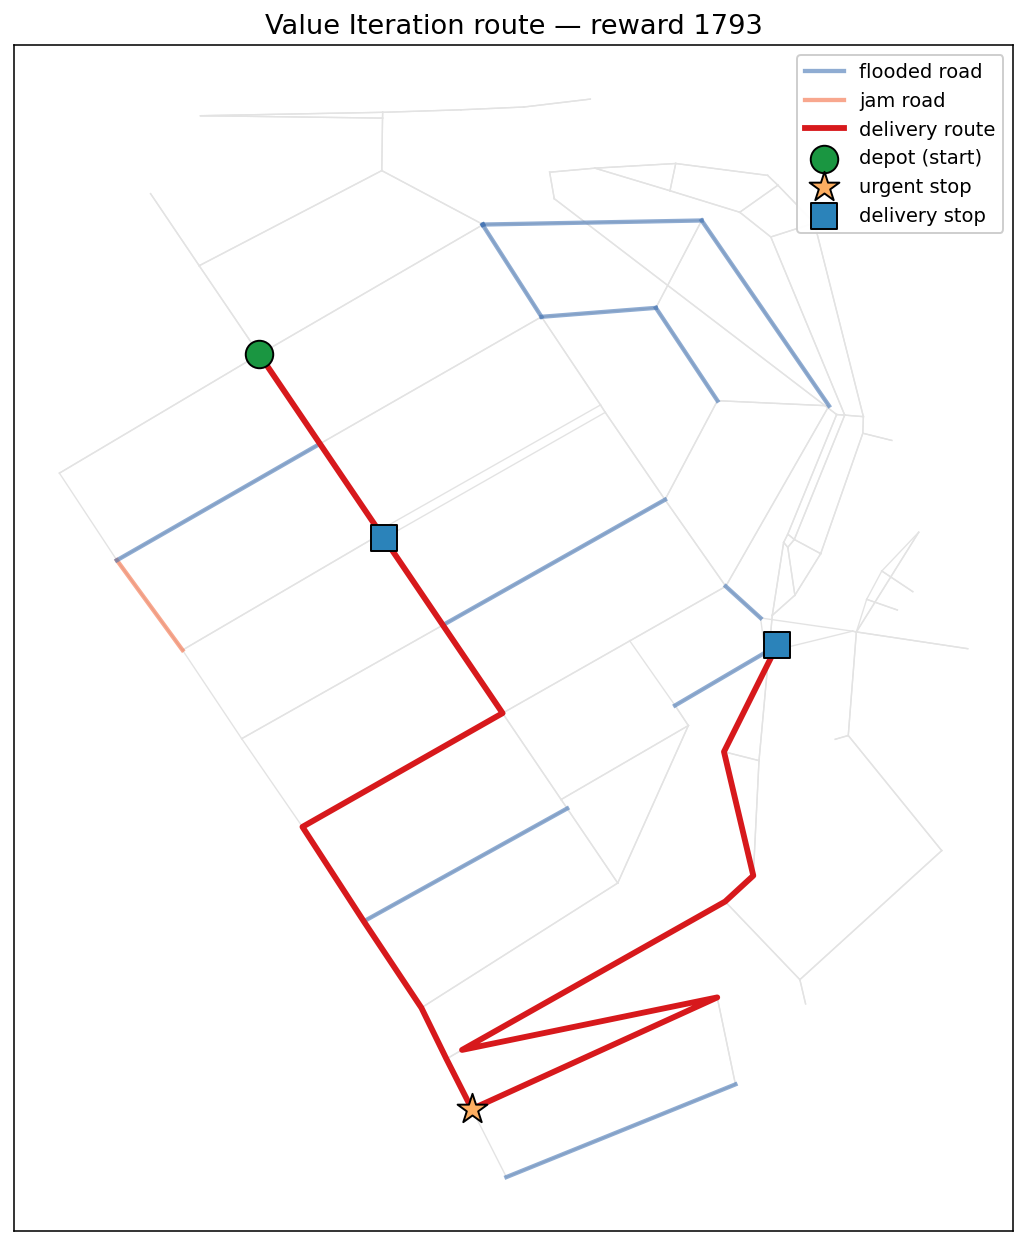
\includegraphics[width=\linewidth]{figures/a4_route_vi.png}
    \caption{Optimal delivery route (urgent stop first).}
  \end{subfigure}\hfill
  \begin{minipage}[t]{0.54\linewidth}
    \vspace{0pt}
    \begin{subfigure}{\linewidth}
      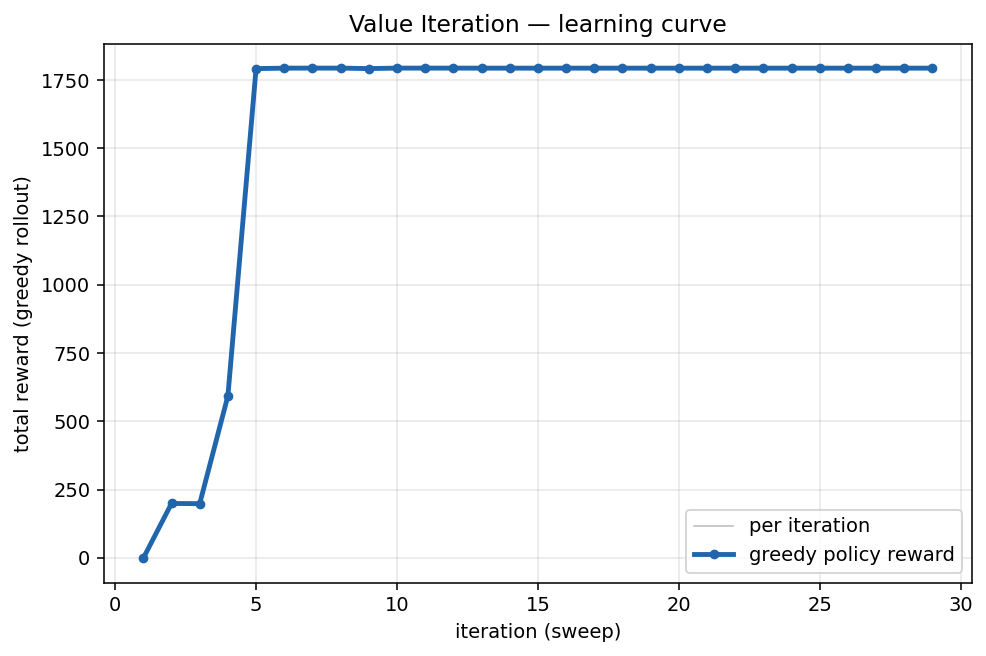
\includegraphics[width=\linewidth]{figures/a4_vi_learning_curve.png}
      \caption{Value Iteration convergence (reward per sweep).}
    \end{subfigure}

    \vspace{0.6em}

    \begin{subfigure}{\linewidth}
      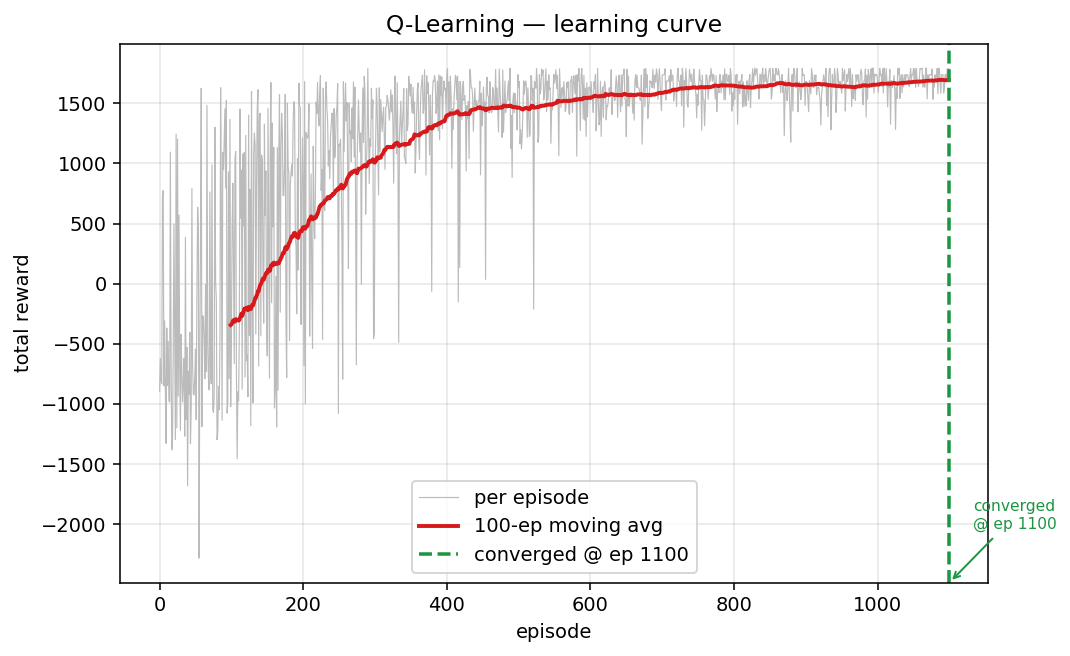
\includegraphics[width=\linewidth]{figures/a4_ql_learning_curve.png}
      \caption{Q-Learning learning curve (reward per episode).}
    \end{subfigure}
  \end{minipage}
  \caption{Worked test case (Dhanmondi, $3$ stops, $1$ urgent): the policy routes through jammed (orange) and flooded (blue) roads to deliver the urgent stop first (left); Value Iteration converges in a few dozen sweeps while Q-Learning climbs to the same reward over thousands of episodes (right).}
  \label{fig:a4}
\end{figure}


\paragraph{Aggregate Analysis} 
\mbox{}\\
We now generalize from this single run to controlled sweeps that vary one factor at a time, examining three aspects: model-free versus model-based cost, sensitivity to the discount $\gamma$, and urgency, stops, and tractability.

\paragraph{Model-free recovers model-based, at a compute premium.}
The tie previewed above holds across every configuration (\Cref{tab:a4}): Value Iteration and Q-Learning converge to essentially the same route reward at each setting, and both always deliver the urgent stop first confirming that a model-free learner, given enough experience, recovers the model-based optimum and that reward-plus-discounting correctly encodes urgency without a deadline. The invariant difference is cost: the ${\sim}20\times$ compute premium of Q-Learning over Value Iteration is the classic model-based/model-free trade-off~\citep{sutton2018rl}.

\paragraph{The discount $\gamma$ is the critical knob.}
$\gamma$ governs foresight, and it is the most sensitive hyper-parameter (\Cref{tab:a4gamma}). At $\gamma=0.5$ the distant $+1000$ terminal reward is discounted into near-irrelevance, so \emph{both} agents turn myopic (reward collapses to $399$). More strikingly, at $\gamma=0.8$ Value Iteration is fine ($1788$) but Q-Learning \emph{destabilizes} to $399$: with a moderate discount and a fixed learning rate, the bootstrapped $Q$ targets fail to propagate the sparse terminal reward reliably within the episode budget a concrete, honest illustration that model-free learning is more fragile to hyper-parameters than exact planning. From $\gamma\ge0.9$ both agree again.

\begin{table}[H]
\centering
\begin{minipage}[t]{0.46\linewidth}
\centering
\small
\begin{tabularx}{\linewidth}{@{}Xrr@{}}
\toprule
$\gamma$ & VI reward & QL reward \\
\midrule
$0.50$ & $399$  & $593$ \\
$0.80$ & $1788$ & $\mathbf{399}$ \\
$0.90$ & $1787$ & $1785$ \\
$0.95$ & $1787$ & $1785$ \\
$0.99$ & $1787$ & $1787$ \\
\bottomrule
\end{tabularx}
\caption{Discount $\gamma$ sweep. QL destabilizes at $\gamma{=}0.8$.}
\label{tab:a4gamma}
\end{minipage}\hfill
\begin{minipage}[t]{0.5\linewidth}
\centering
\small
\begin{tabularx}{\linewidth}{@{}Xrr@{}}
\toprule
Setting & VI & QL \\
\midrule
baseline ($3$ stops) & $1787$ & $1785$ \\
$2$ stops ($352$ states) & $1596$ & $1596$ \\
$4$ stops ($1408$ states) & $1987$ & $1987$ \\
$0$ urgent & $1587$ & $1587$ \\
$2$ urgent & $1987$ & $1987$ \\
\bottomrule
\end{tabularx}
\caption{VI vs.\ QL agree across stops and urgency (reward; iters/episodes).}
\label{tab:a4}
\end{minipage}
\end{table}

\paragraph{Urgency, stops, and tractability.}
Reward scales interpretably (\Cref{tab:a4}): each additional stop adds ${\sim}200$ ($1596\to1787\to1987$ for $2\to3\to4$ stops), and converting a normal stop to urgent adds another ${\sim}200$ ($1587\to1787\to1987$ for $0\to1\to2$ urgent), exactly as the reward table dictates, with the urgent stop always served first. The results are robust across seeds ($1787$--$1794$) and hazard densities ($1792$/$1787$/$1788$ for low/medium/high). The cost of the extra stop is state-space growth: the state count $|V|\cdot2^{K}$ rises from $352$ to $1408$ as $K$ goes $2\to4$, which is why $K$ must stay small for exact Value Iteration the practical ceiling of a tabular method.

\subsection{Key Takeaways and Empirical Synthesis}
This assignment contrasts planning and learning on one stochastic problem. Given the model, Value Iteration plans the optimal delivery policy in a few dozen sweeps; without the model, Q-Learning learns the \emph{same} policy including urgent-first delivery from experience alone, but at ${\sim}20\times$ the compute and with greater hyper-parameter fragility, exposed by its $\gamma{=}0.8$ collapse where the exact planner is untroubled. Reward magnitude plus discounting encodes urgency correctly without a state-expanding deadline, and reward scales interpretably with stops and urgency. The discount $\gamma$ is the decisive knob, and the tabular state count $|V|\cdot2^{K}$ is the scalability ceiling the point at which one would move from exact Value Iteration to function-approximation reinforcement learning.

% =====================================================================
\section{Conclusions}
\label{sec:conclusion}
Holding the domain fixed  the Dhaka road network  and varying the
Artificial Intelligence paradigm produced four findings that
reinforce one another.

In \textbf{search} (Section~\ref{sec:search}), $A^{*}$ matched the
uniform-cost optimum while expanding $4.7\times$ fewer nodes
($7{,}519$ versus $35{,}496$), but a controlled two-setup
comparison showed that this advantage is not a property of $A^{*}$
at all: replacing the reverse-Dijkstra lower bound with a
geometry-only Euclidean heuristic  blind to traffic and safety,
the terms that dominate the cost surface  collapsed $A^{*}$ onto
uniform-cost search ($35{,}116$ expansions) and inflated greedy
best-first's solution cost more than fourfold. Informed search is
worth exactly as much as its heuristic's fidelity to the true cost,
and no more.

In \textbf{constraint satisfaction} (Section~\ref{sec:csp}), AC-3
propagation with MRV, degree, and LCV ordering plus forward
checking converted a $601{,}618$-backtrack timeout into a
zero-backtrack solve at $n = 70$, yet systematic search still hit
an absolute wall by $n = 100$, where only Min-Conflicts returned a
usable assignment. An ablation on a deliberately infeasible
instance sharpened the lesson: ordering and lookahead accelerate
\emph{finding} a solution but do nothing to accelerate
\emph{proving} that none exists. At city scale the framework acted
less as a solver than as a policy validator, showing that strict
plate-parity, emergency reserves, and queue caps leave $118$ of
$150$ users unassignable before search even begins  a limit of the
rationing policy, not of the algorithm.

In \textbf{population-based optimisation}
(Section~\ref{sec:swarm}), the honest result is that on plain
submodular coverage a greedy baseline is already near-optimal by
the classic $1 - 1/e$ guarantee, and all three warm-started
metaheuristics could only tie it. The swarm advantage appeared only
once an overlap penalty made the objective non-submodular
\emph{and} a continuous decision variable was available: Particle
Swarm Optimisation, alone in optimising the facing angle
continuously, overtook greedy at every penalty level, while the
discrete-angle Genetic Algorithm and Ant Colony Optimisation did
not. The adversarial greedy-fail scenario isolated the mechanism
precisely  greedy's wasted overlap stayed pinned near $4.5\%$
while PSO drove it below $1.5\%$.

In \textbf{reinforcement learning} (Section~\ref{sec:rl}),
model-based Value Iteration and model-free Q-Learning converged to
the same optimal policy, both serving the urgent delivery first,
confirming that reward magnitude combined with discounting encodes
urgency without a state-expanding deadline. The invariant
difference was cost: Q-Learning paid a ${\sim}20\times$ compute
premium for not being handed the model, and proved measurably more
fragile, destabilising at $\gamma = 0.8$ where the exact planner
was untroubled.

\paragraph{The unifying lesson.} Algorithm selection should follow
problem structure rather than habit or novelty:
\emph{informativeness} for heuristic search, \emph{propagation and
scale} for constraint reasoning, \emph{submodularity and parameter
continuity} for optimisation, and \emph{model availability under
uncertainty} for sequential decision making. In three of the four
cases the sophisticated method earned its keep only when a specific
structural property defeated the simpler baseline's guarantee;
recording the cases where it did \emph{not} is as much a result as
recording the cases where it did.

\paragraph{Limitations.} Three deserve emphasis. First, several
components of the environment are synthesised because open Dhaka
data at edge-level granularity does not exist  station capacities,
the crime and crowd risk field, hazard placement, and the traffic
and safety proxies of the routing study  so the absolute cost and
coverage magnitudes given here are not measurements. Second, the
Markov decision process is kept deliberately small
($|V| \cdot 2^{K}$ states) to keep tabular Value Iteration exact,
which caps the number of delivery stops well below an operational
fleet's. Third, the coverage model treats visibility as a clean
geometric cone with no occlusion, which overstates achievable
coverage in the dense, irregular built form of Old Dhaka in
particular.

\paragraph{Future work.} The natural extensions follow directly
from those limitations: substituting real incident and crash
records for the synthetic risk field and calibrating the cost model
against measured travel times; adding line-of-sight occlusion, and
ideally building-footprint geometry, to the coverage objective; and
replacing tabular Value Iteration with function-approximation
reinforcement learning to lift the state-space ceiling on the
delivery task and admit a realistic number of stops. A further
direction is to relax the assumption that the four problems are
independent: in a real deployment the routing, rationing,
surveillance, and delivery decisions share the same congested
network and could be posed jointly.
\bibliographystyle{plainnat}
\bibliography{references}

\end{document}
